\chapter{Scattering cross--section} 

\section{Position of the problem} 
%theoretical description - implementation in \BornAgain
%Influence / contribution of particles (form factor) and sample geometry, interferences between particles, layer roughness,...
%Modelling in grazing incidence : DWBA, BA, level of approximation
%In GISAS experiments, information on the sizes, shapes of the scatterers as well as information on their relative distributions can be obtained.

This section describes how assemblies of particles and layers of materials contribute to the scattering cross--section \textit{i.e.} the way their spatial distributions and the distribution of shapes and their correlations or layers' roughness can influence the output intensity. 

The samples generated with \BornAgain\ are made of different layers of materials characterized by their thicknesses, refractive indices, and possible surface roughnesses. Except for the thickness, the other dimensions of the layers are infinite.\\ Particles can be embedded in or deposited on the top of any layers. Those particles are characterized by their shapes, refractive indices, their spatial distribution and concentration in the sample. The influence of the particles' shapes is described by the form factors. When the particles are densely packed, the distance relative to each other becomes of the same order as the particles' sizes. The radiation scattered from these various particles are going to interfere together. \\ We are first going to give a short overview of the theory involved, mostly in order to define the terminology. For a more complete theoretical description, the user is referred to, for example, reference~\cite{ReLa09} and appendix \ref{appendixtheory} of this manual. Then we are going to describe how the interference features, the form factors and the characteristics of the material layers have been implemented in \BornAgain\ and  give some examples.

%%%%%%%%%%%%%%%%%%%%%%%%%%%%%%%%%%%%%%%%
\section{Collection of particles} \SecLabel{sect:interf}
Let us consider the general geometry of a scattering experiment. An incident neutron with a wave vector $\mathbf{k}_i$ is scattered in a new direction $\mathbf{k}_f$ after interacting with a particle. This scattering occurs in a cone of solid angle $d\Omega$ around the direction of the scattered wave vector $\mathbf{k}_f$.
Considering a set of $N$ particles labeled with index $i$, located at $\mathbf{R}_i$ and having shapes $S_i(\mathbf{r})$ ($S_i=0$ outside the particle and 1 inside), occupying a total volume $V$, the differential cross--section per particle is given by:
\begin{equation*}
  \frac{d\sigma}{d\Omega}(\vect{q}) = \frac{1}{N}\left\lbrace \sum_i \left\lvert F_i(\vect{q}) \right\rvert ^2 + \sum_{i\neq j} F_i(\vect{q}) F_{j}^*(\vect{q}) \exp \left[i\vect{q}\cdot (\vect{R}_i-\vect{R}_j)\right] \right\rbrace \; .
\end{equation*}
where  $\mathbf{q}=\mathbf{k}_i - \mathbf{k}_f$ is the wave vector transfer and $F_i$ is the form factor of particle $i$ (see \SecRef{sect:ff} for a description).


Since in most experimental conditions only the statistical properties of the particles are known, one can consider the probabilistic value of this cross--section \textit{i.e.} its expectation value. Assuming that the particles' shapes are determined by their class $\alpha$, with the abundance ratio $p_\alpha \equiv N_\alpha / N$, and defining the particle density as $\rho_V \equiv N/V$, the expectation value becomes:
\begin{align*}
  \left\langle \frac{d\sigma}{d\Omega}(\vect{q}) \right\rangle  & = \sum_\alpha p_\alpha \left\lvert F_\alpha(\vect{q})\right\rvert ^2 + \frac{\rho_V}{V}\sum_{\alpha,\beta} p_\alpha p_\beta F_\alpha (\vect{q})F_\beta^*(\vect{q})  \\
  & \times \iint_V d^3\vect{R}_\alpha d^3\vect{R}_\beta \ppcf{\alpha}{\beta}{R} \exp \left[ i\vect{q}\cdot (\vect{R}_\alpha - \vect{R}_\beta ) \right] \; ,
\end{align*}

where $\ppcf{\alpha}{\beta}{R}$ is called the \emph{partial pair correlation function}. It represents the normalized probability of finding particles of type $\alpha$ and $\beta$ in positions $\vect{R}_\alpha$ and $\vect{R}_\beta$ respectively. 
%\begin{equation}
%  \frac{d\sigma(\mathbf{q})}{d\Omega} = \frac{1}{N}\left\langle \left\lvert \sum_i F^i(q)e^{i \mathbf{q}\cdot \mathbf{R}_i}\right\rvert^{2} \right\rangle =\frac{1}{N}\left\langle \sum_i |F_i(\mathbf{q})|^2+\sum_{i \neq j} F_i(\mathbf{q}) F_j ^*(\mathbf{q})\exp(i\mathbf{q}\cdot (\mathbf{R}^i-\mathbf{R}^j)) \right\rangle, \label{eq:interfintensity}
%\end{equation}
%where $\langle\ldots\rangle$ denotes a spatial and temporal average, $\mathbf{q}$ is the wave vector (in reciprocal space) and $F^i$ is the form factor of particle $i$. 

%If only the statistical quantities of the system are known (particles' positions and sizes), the discrete sums in equation~\ref{eq:interfintensity} can be replaced by continuous integrals using some probability densities. For example, in two dimensions (which is the case for particles deposited on a surface), the probability per unit surface to find a particle of class $\alpha$ in $\mathbf{R}_{i}$ knowing that there is a particle of type $\beta$ in $\mathbf{R}_{j}$ can be written as  $\rho_S^2 g_{\alpha \beta}(R_{i,\alpha},R_{j,\beta})$ where $\rho_S$ is the number of particles  per unit surface and $g_{\alpha \beta}$ is the partial pair correlation function, which tends towards 1 as the distance between the particles increases.
%%%%%%%%%%%%%%%%%%%%%%%%%%%%%%%%%%%%%%%%
\subsection{Size-distribution models}

To proceed further, when the morphology and topology are not exactly known, some hypotheses need to be made since the correlation between the kinds of scatterers and their relative positions included in the pair correlation functions are difficult to estimate. Several options are available:

\paragraph{Decoupling approximation (DA)} neglects all correlations. It supposes that the particles are positioned in a way that is completely independent on their kinds (shapes, sizes). Thus the kind of scattering objects and their positions are not correlated and the partial pair correlation function is independent of the particle class $\alpha$. We can therefore replace $ \ppcfb{\alpha}{\beta}{R}$ by  $g(\vect{R}_{\alpha\beta})$.

This leads to the following expression of the scattering cross--section:
\begin{equation*}
\left\langle \frac{d\sigma}{d\Omega}(\vect{q}) \right\rangle  = I_d(\vect{q}) + \left\lvert \left\langle F_\alpha(\vect{q}) \right\rangle_\alpha \right\rvert ^2 \times S(\vect{q}) \; ,
\end{equation*}
where $S(\vect{q})$ is the interference function and is given by
\begin{equation*} 
  S(\vect{q}) = 1+ \rho_V \int_V d^3\vect{R} \; g(\vect{R}) \exp \left[ i\vect{q}\cdot \vect{R} \right] \; .
\end{equation*}

In concentrated systems, DA breaks down because of correlations. One solution is to reintroduce some correlations between particles sizes and distributions using, for example, the size spacing correlation approximation described below. 

\paragraph{Local monodisperse approximation (LMA)} partially accounts for some coupling between the positions and the kinds of the particles \cite{Pede94}. 
 It requires a subdivision of the layers of particles into monodisperse domains. The contributions of these subdomains are then  incoherently summed up and weighted by the size-shape probabilities.\\ In this approximation, a particle is supposed to be surrounded by particles of the same size and shape, within the coherence length of the input beam. The scattering cross--section is expressed as
\begin{equation*}
  \left\langle \frac{d\sigma}{d\Omega}(\vect{q}) \right\rangle \simeq \left\langle \left\lvert F_\alpha(\vect{q})\right\rvert ^2 S_\alpha(\vect{q}) \right\rangle_\alpha \; .
\end{equation*}

Contrary to the Decoupling Approximation, the Local Monodisperse Approximation can account for particle class/size/shape--dependent pair correlation functions by having distinct interference functions $S_\alpha(\vect{q})$.

One has to remember that in most cases, this approximation corresponds to an unphysical description of the investigated systems. \\ 

DA and LMA separate the contributions of the form factors and of the interference function. For disordered systems DA and LMA give the same result as the scattering vector gets larger \textit{i.e.} the scattered intensity is dominated by the contribution of the form factor.

\paragraph{Size spacing correlation approximation (SSCA)} introduces correlations between polydisperse particles, more precisely between the shape/size of the particles and their mutual spacing. A classical example would consist of particles whose closest--neighbour spacing depends linearly on the sum of their respective sizes \cite{LaLe07}.

For a sample where only the statistical properties of particle positions and shape/size are known, the scattered intensity per scattering particle is expressed as the average over an ensemble of the Fourier transform of the Patterson function, which is the autocorrelation of the scattering length density $\curlp (\vectr ) \equiv \sum_{ij} S_i(-\vectr )\otimes S_j(\vectr )\otimes \delta (\vectr + \vectr_i - \vectr_j )$:
\begin{equation*}
  I(\vectq ) = \frac{1}{N}\ensavg{}{\curlf (\curlp (\vectr ))} \; ,
\end{equation*}
where $\curlf$ denotes the Fourier transform and $\curlp$ the Patterson function.\\



\MakeRemark{Terminology}{
\\
For collections of particles, the scattered intensity contains contributions from neighboring particles. This additional pattern can be called the structure factor, the interference function or even in crystallography, the lattice factor. In this manual, we use the term "interference function" or interferences.
}

%%%%%%%%%%%%%%%%%%%%%%%%%%%%%%%%%%%%%%%%
\subsection{Layout of particles}\label{sec:partlayout}

\subsubsection{The uncorrelated or disordered lattice}
For very diluted distributions of particles, the particles are too far apart from each other to lead to any interference between the waves scattered by each of them. In this case the interference function is equal to 1. The scattered intensity is then entirely determined by the form factors of the particles distributed in the sample.

\subsubsection{The regular  lattice}\mbox{}\\
The particles are positioned at regular intervals generating a layout characterised by its base vectors $\mathbf{a}$ and $\mathbf{b}$ (in direct space) and the angle between these two vectors.
This lattice can be two or one-dimensional depending on the characteristics of the particles. For example when they are infinitely long, the implementation can be simplified and reduced to a "pseudo" 1D system.

\paragraph{The ideal paracrystal} \mbox{}\\
A paracrystal, whose notion  was developed by Hosemann\cite{Hos51}, allows fluctuations of the lengths and orientations of lattice vectors. Paracrystals can be defined as distorted crystals in which the crystalline order has not disappeared and for which the behavior of the interference functions  at small angles is coherent.
It is a transition between the regular lattice and the disordered state.\\


For example, in one dimension, a paracrystal is generated using the following method. First we place a particle at the origin. The second particle is put at a distance $x$ with a density probability $p(x)$ that is peaked at a mean value $D$: $\int_{-\infty} ^{\infty}p(x)dx=1$ and $\int_{-\infty}^{\infty}xp(x)dx=D$. The third one is added at a distance $y$ from the second site using the same rule with a density probability $p_2(y)= \int_{-\infty}^{\infty}p(x)p(y-x)dx=p\otimes p(y)$.\\ With such a method, the pair correlation function $g(x)$ is built step by step. Its expression and the one of its Fourier transform, which is the interference function are 
\begin{equation*}
g(x)=\delta(x)+ p(x)+ p(x)\otimes p(x)+\ldots + p(-x)+\ldots \: \mathrm{and}\:\, S(q)=\Re\left(\dfrac{1+P(q)}{1-P(q)}\right),
\end{equation*}
 where $P(q)$ is the Fourier transform of the density probability $p(x)$.\\


In two dimensions, the paracrystal is constructed on a pseudo-regular lattice with base vectors $\mathbf{a}$ and $\mathbf{b}$ using the following conditions for the densities of probabilities:\\ $\int p_{\mathbf{a}}(\mathbf{r})d^2\mathbf{r}=\int p_{\mathbf{b}}(\mathbf{r})d^2\mathbf{r}=1$, $\int \mathbf{a} p_{\mathbf{a}}(\mathbf{r})d^2\mathbf{r}=\mathbf{a}$, $\int \mathbf{b} p_{\mathbf{b}}(\mathbf{r})d^2\mathbf{r}=\mathbf{b}$.\\
In the ideal case the two axes are decoupled and each unit cell should retain a parallelogram shape. The interference function is given by $S(q_{\parallel})=\prod_{k=a,b}\Re\left(\dfrac{1+P_k(q_{\parallel})}{1-P_k(q_{\parallel})} \right)$ with $P_k$ the Fourier transform of $p_k$, $k=a, b$.

\paragraph{Probability distributions} \label{baftd} \mbox{}\\
The scattering by an ordered lattice gives rise to a series of Bragg peaks situated at the nodes of the reciprocal lattice. Any divergence from the ideal crystalline case modifies the output spectrum by, for example, widening or attenuating the Bragg peaks. The influence of these "defects" can be accounted for 
 in direct space using correlation functions or by truncating the lattice or, in reciprocal space with structure factors or interference functions by convoluting the scattered pics with a function which could reproduce the experimental shapes.

%%%%%%%%%%%%%%%%%%%%%%%%%%%%%%%%%%%%%%%%
\subsection{Implementation in \BornAgain}

This section describes the implementation of the interference functions in \BornAgain. For an implementation of all the components of a simulation, the use is referred, for example, to \SecRef{Example1Python}.\\


\ImportantPoint{Remark:}{In \BornAgain\ the particles are positioned in the same vertical layer.}

\subsubsection{Size-distribution models}
The decoupled approximation, local monodisperse approximation and size spacing correlation approximation can be used in \BornAgain.
The selection is made using \Code{SimulationParameters()} when defining the characteristics of the simulation.  For example,
\begin{lstlisting}[language=python, style=eclipseboxed,numbers=none,nolol]
    simulation = Simulation()
   ....
    sim_params = SimulationParameters()
# interference approx chosen between: DA (default), LMA and SSCA
    sim_params.me_if_approx = SimulationParameters.LMA
    simulation.setSimulationParameters(sim_params)
\end{lstlisting}

%The users can refer to Script~\ref{lst:2dlatticeinterf} for a more detailed implementation. By default, the decoupled approximation (DA) is used.

%%%%%%%%%%%%%%%%%%%%%%%%%%%%%%%%%%%%%%%%
\subsubsection{Probability distribution functions}\label{baftd}
The probability distribution functions have been implemented in the reciprocal space in \BornAgain. Their expressions are given in Table~\ref{table:pdf}.

\begin{table}[H]
\centering
\begin{tabular}{ccc}
\hline 
Function & One dimension & Two dimensions\\
\hline 
Cauchy & $(1+q^2\omega^2)^{-3/2}$ & $(1 + q_x^2 cl_x^2 + q_y^2 cl_y^2)^{-3/2}$ \\
Gauss & $\dfrac{1}{2}\exp(-\dfrac{q^2\omega^2}{4})$ & $\frac{1}{2}\exp\left(-\dfrac{q_x^2 cl_x^2+ q_y^2cl_y^2}{4}\right)$ \\
Voigt & $\dfrac{\eta}{2} \exp\left(-\dfrac{q^2\omega^2}{4}\right) + \dfrac{1 - \eta}{(1 + q^2\omega^2)^{3/2}}$ & $\dfrac{\eta}{2} \exp\left(-\dfrac{q_x^2 cl_x^2+ q_y^2cl_y^2}{4}\right)+ \dfrac{1 - \eta}{(1 + q_x^2 cl_x^2+ q_y^2cl_y^2)^{3/2}}$ \\
\hline
\end{tabular}
\caption{List of probability distribution functions in reciprocal space. $\omega$, $cl$ stand for coherence lengths (the index refers to the axis) and  $\eta$ is a weighting coefficient.}
\label{table:pdf}
\end{table}

The Cauchy distribution corresponds to $\exp(-r)$ in real space and the Voigt one  is a linear combination of the Gaussian and Cauchy probability distribution functions.\\

\noindent \underline{One dimension}
\begin{itemize}
\item \Code{FTDistribution1DCauchy($\omega$)},
\item \Code{FTDistribution1DGauss($\omega$)},
\item \Code{FTDistribution1DVoigt($\omega, \eta$)}.
\end{itemize}
where $\omega$ is the coherence length and $\eta$ is a weighting factor.\\

\noindent \underline{Two dimensions}
\begin{itemize}
\item \Code{FTDistribution2DCauchy($cl_x$, $cl_y$)},
\item \Code{FTDistribution2DGauss($cl_x$, $cl_y$)},
\item \Code{FTDistribution2DVoigt($cl_x$, $cl_y$)}
\end{itemize}
where $cl_{x,y}$ are the coherence lengths in the $x$ or $y$ direction, respectively.

These functions can be used with all interference functions except the case without any interference and the one dimensional paracrystal, for which only the Gaussian case has already been implemented.
%%%%%%%%%%%%%%%%%%%%%%%%%%%%%%%%%%%%%%%%
\subsubsection{Interferences}

The interference function is specified when building the sample. It is linked with the particles (shape, material). Examples of implementation are given at the end of each description.

\paragraph{Syntax:}
 \Code{particle\_layout.addInterferenceFunction(interference\_function)},\\ where \Code{particle\_layout} holds the information about the different shapes and their proportions for a given layer of particles, and \Code{interference\_function}  is one of the following expressions:
\begin{itemize}
\item \Code{InterferenceFunctionNone()}
\item \Code{InterferenceFunction1DLattice(lattice\_parameters)}
\item \Code{InterferenceFunction1DParaCrystal(peak\_distance, width,corr\_length)}
\item \Code{InterferenceFunction2DLattice(lattice\_parameters)}
\item \Code{InterferenceFunction2DParaCrystal(length\_1, length\_2, $\alpha$\_lattice, $\xi$, \\ damping\_length)}
\end{itemize}



\ImportantPoint{Remark:}{\Code{InterferenceFunction1DLattice} can only be used for particles which are infinitely long in one direction of the sample's surface like for example a rectangular grating.}

\newpage
%%%%%%%%%%%%%%%%%%%%%%%%%%%%%%%%%%%%%%%%%%
\subsubsection{\ding{253} \Code{InterferenceFunctionNone()}} 
The particles are placed randomly in the dilute limit and are considered as individual, non-interacting scatterers. The scattered intensity is function of the form factors only. 

\paragraph{Example} The sample is made of a substrate on which are deposited half-spheres. Script~\ref{lst:nointerf} details the commands necessary to generate such a sample. Figure~\ref{fig:nointerf} shows an example of output intensity: Script~\ref{lst:nointerf}  + detector + input beam. The full script UMInterferencesNone.py can be found in /Examples/python/UserManual. 


\begin{figure}[h]
\begin{center}
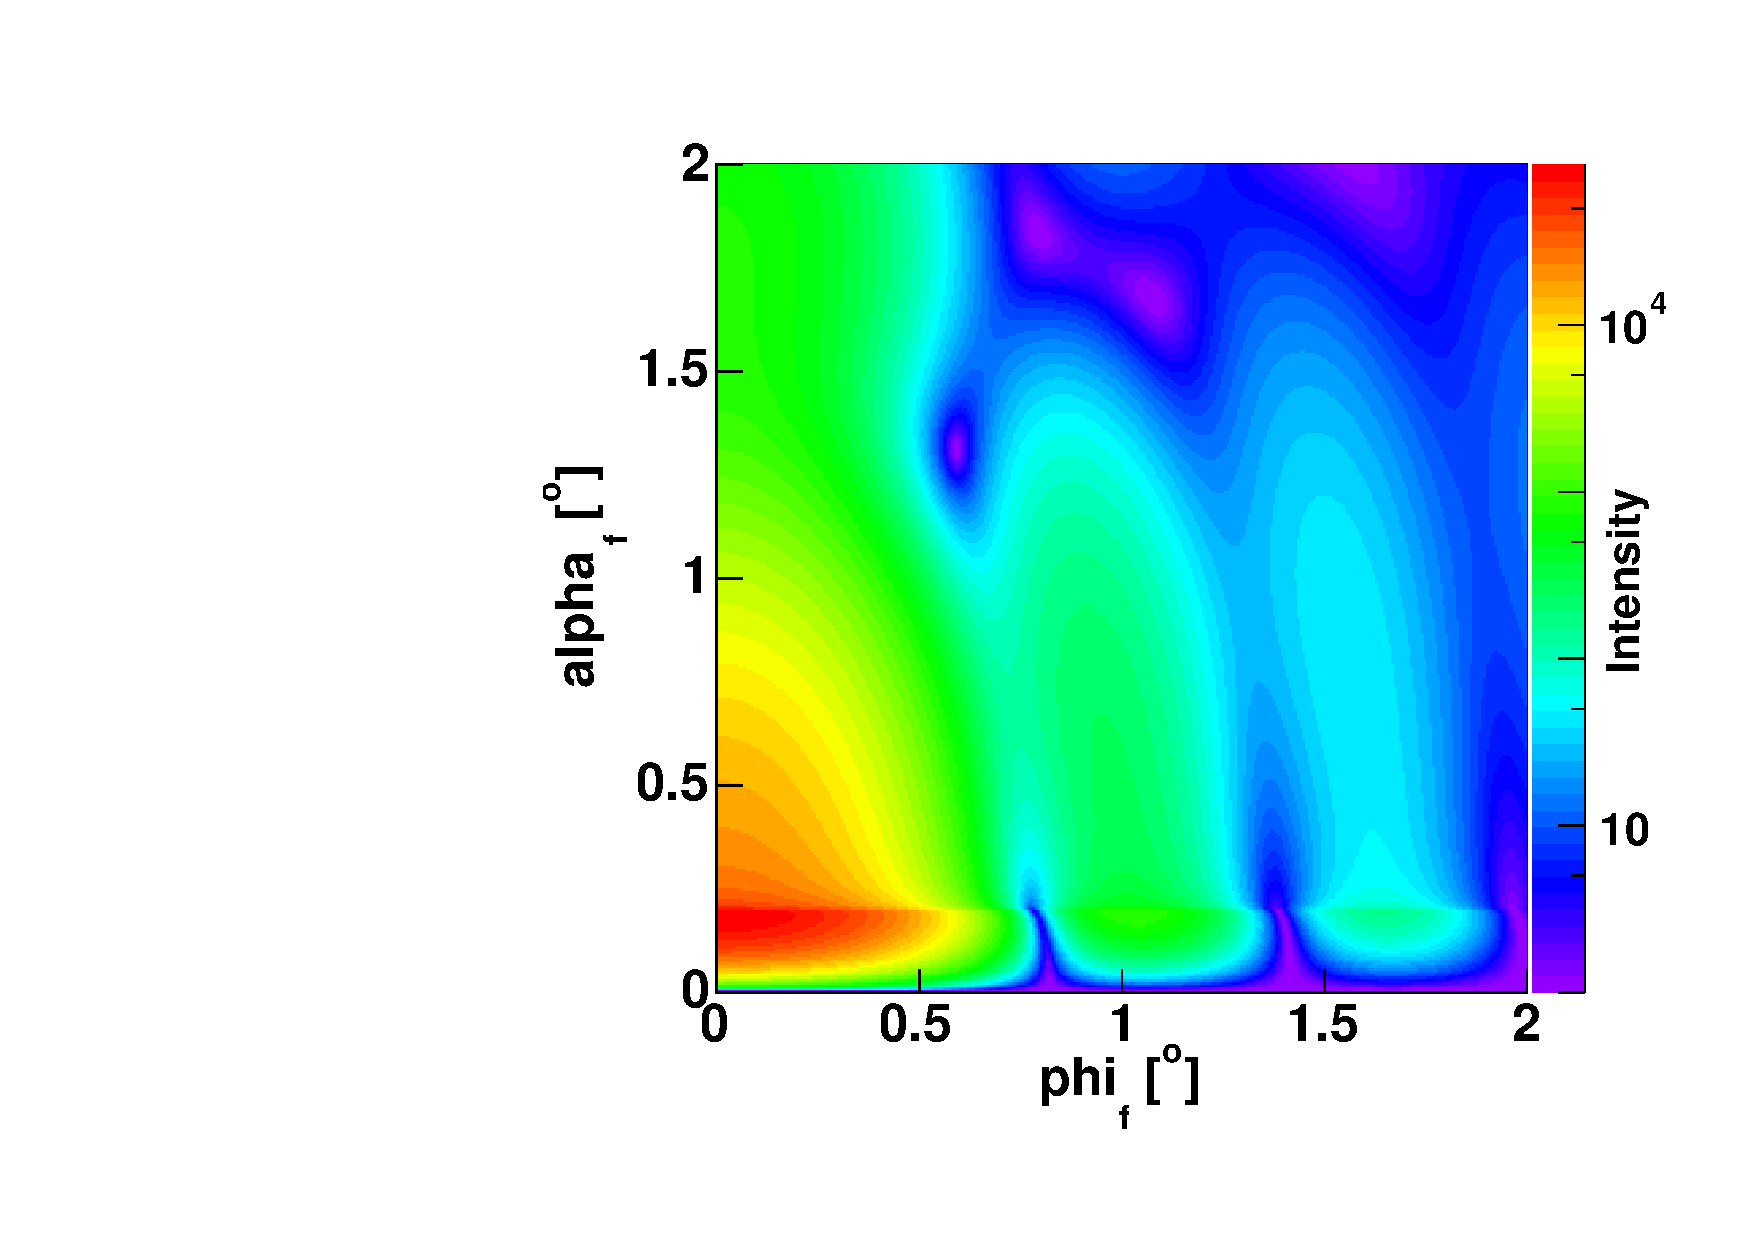
\includegraphics[width=0.5\textwidth]{Figures/HSphere_NoInterf}
\end{center}
\caption{Output intensity scattered from a sample made of half-spheres with no interference between them.}
\label{fig:nointerf}
\end{figure}

\FloatBarrier
\newpage

\begin{lstlisting}[language=python, style=eclipseboxed,numbers=none,nolol,caption={\Code{Python} script to simulate a sample made of half-spheres deposited on a substrate layer without any interference. The part specific to the interferences is marked in red italic font.},label={lst:nointerf}]
def get_sample():
    """
    Build and return the sample representing particles with no interference
    """
    # defining materials
    m_ambience = HomogeneousMaterial("Air", 0.0, 0.0)
    m_substrate = HomogeneousMaterial("Substrate", 6e-6, 2e-8)
    m_particle = HomogeneousMaterial("Particle", 6e-4, 2e-8)
    # collection of particles
    sphere_ff = FormFactorTruncatedSphere(5*nanometer, 5*nanometer)
    sphere = Particle(m_particle, sphere_ff)
    particle_layout = ParticleLayout()
    particle_layout.addParticle(sphere, 0.0, 1.0)
    |interference = InterferenceFunctionNone()| 
    |particle_layout.addInterferenceFunction(interference)|
    # assembling the sample
    air_layer = Layer(m_ambience)
    air_layer.setLayout(particle_layout)
    substrate_layer = Layer(m_substrate, 0)

    multi_layer = MultiLayer()
    multi_layer.addLayer(air_layer)
    multi_layer.addLayer(substrate_layer)
    return multi_layer
\end{lstlisting}

\newpage{\cleardoublepage}
%%%%%%%%%%%%%%%%%%%%%%%%%%%%%%%%%%%%%%%%%%
\subsubsection{\ding{253}  \Code{InterferenceFunction1DLattice(lattice\_parameters)}} 
where  \Code{lattice\_parameters}=(lattice\_length, $\xi$) with lattice\_length is the lattice constant and $\xi$ the angle in radian between the lattice unit vector and the $\mathbf{x}$-axis of the "GISAS experiment" referential as shown in fig.~\ref{fig:1dgrating}.

\begin{figure}[h]
\begin{center}
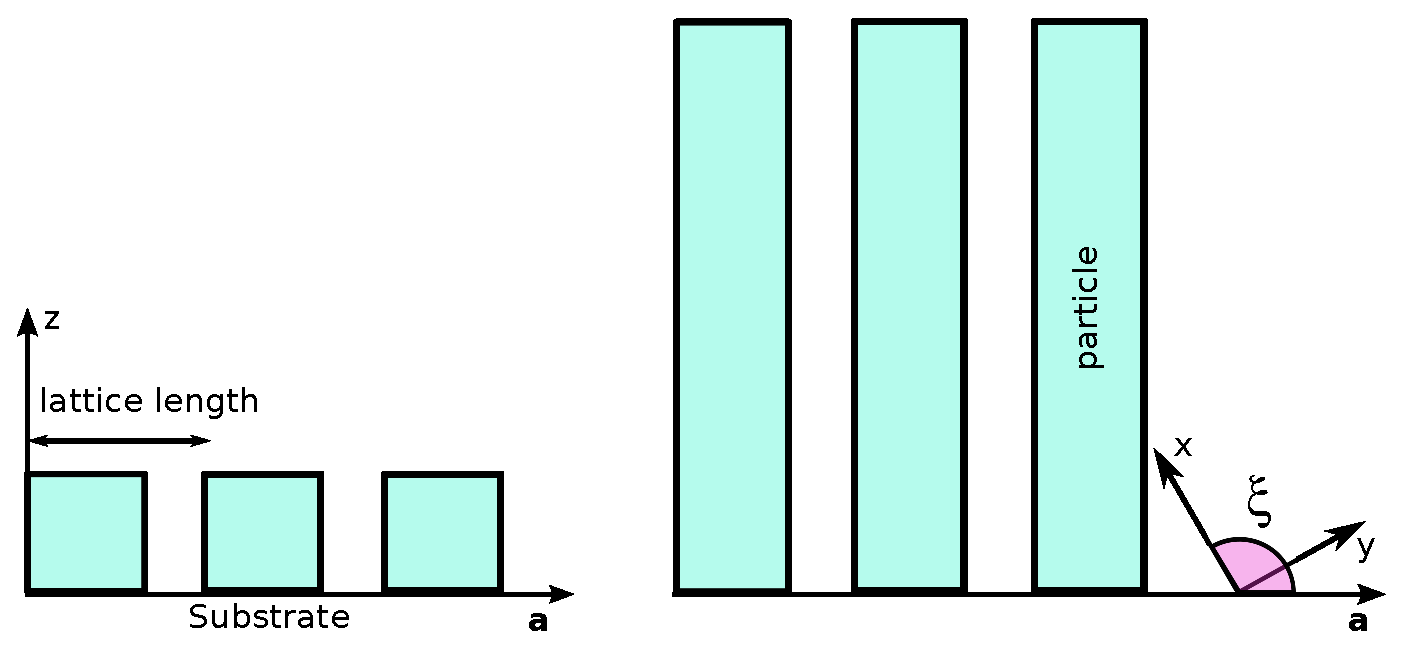
\includegraphics[width=0.75\textwidth]{Figures/1DGrating}
\end{center}
\caption{Schematic representation of a 1D lattice (side and top views). Such a lattice is characterized by a lattice length and the angle $\xi$.}
\label{fig:1dgrating}
\end{figure}

\ImportantPoint{Remark:}{By default the long axis of the particles in this 1D lattice is along the beam axis: $\xi=90^{\circ}$.}

\vspace{12pt}
A probability distribution function \Code{pdf} has to be chosen from the list in section~\ref{baftd} in order to apply some modifications to the scattering peaks. This function is implemented using \Code{setProbabilityDistribution(pdf)}. 

\paragraph{Example:} Instead of giving a full script to generate the scattered intensity plot, we are focusing on how to build a sample using \Code{InterferenceFunction1DLattice} as the interference function in \BornAgain .\\ Script~\ref{lst:1dlattinterf} details this procedure in \Code{Python}. As mentioned previously, this interference function can only be used with infinitely wide or long particles.\\ Here the sample is made of infinitely long boxes deposited on a substrate (these particles are characterized by their widths and heights). They are also rotated by $90^{\circ}$  in the sample surface in order to have their long axis perpendicular to the input beam, along the $x$-axis.\\
 The lattice parameters (the lattice lengths and angle between the lattice main axis and the $x$-axis) are specified using \Code{Lattice1DIFParameters()} and are then used as input parameters of the interference function.

\newpage
\begin{lstlisting}[language=python, style=eclipseboxed,numbers=none,nolol,caption={\Code{Python} script to generate a sample made of infinitely long boxes deposited on a substrate layer with the 1DLatticeInterference function. The part specific to the interferences is marked in red italic font.},label={lst:1dlattinterf}]
def get_sample():
    """
    Build and return the sample with 1DLatticeInterference function
    """
    # defining materials
    m_air = HomogeneousMaterial("Air", 0.0, 0.0)
    m_substrate = HomogeneousMaterial("Substrate", 6e-6, 2e-8)
    m_particle = HomogeneousMaterial("Particle", 6e-4, 2e-8)

    # collection of particles
    ff = FormFactorInfLongBox(10.*nanometer, 15.0*nanometer)
    box = Particle(m_particle, ff)
    particle_layout = ParticleLayout()
    transform = Transform3D.createRotateZ(90.0*degree)
    particle_layout.addParticle(box, transform)

    # lattice parameters
    |lattice_params = Lattice1DIFParameters()|
    |lattice_params.m_length = 30.0*nanometer|
    |lattice_params.m_xi = 0.0*degree|

    # interference function
    |interference = InterferenceFunction1DLattice(lattice_params)|
    |pdf = FTDistribution1DCauchy(200./2./M_PI*nanometer)|
    |interference.setProbabilityDistribution(pdf)|
    |particle_decoration.addInterferenceFunction(interference)|

    # air layer with particles and substrate form multi layer
    air_layer = Layer(m_air)
    air_layer.setDecoration(particle_decoration)
    substrate_layer = Layer(m_substrate, 0)

    multi_layer = MultiLayer()
    multi_layer.addLayer(air_layer)
    multi_layer.addLayer(substrate_layer)
    return multi_layer
\end{lstlisting} 

\newpage{\cleardoublepage}
%%%%%%%%%%%%%%%%%%%%%%%%%%%%%%%%%%%%%%%%%%
\subsubsection{\ding{253} \Code{InterferenceFunction1DParaCrystal(peak\_distance, width, corr\_length)}}  
\begin{itemize}
\item[where] \Code{peak\_distance} is the average distance to the first neighbor peak, 
\item[]\Code{width} is the width parameter of the probability distribution,
\item[] \Code{corr\_length} is the correlation length (equal to 0 by default).
\end{itemize}

For this particular interference function, the implemented probability distribution function is Gaussian:

\begin{equation*}
p(x)=\frac{1}{\omega \sqrt{2\pi}} \exp\left(-\dfrac{(x-D)^2}{\omega^2}\right),\qquad P(q_{\parallel})=\exp\left(-\frac{q_{\parallel}^2 \omega^2}{2}\right)\exp(iq_{\parallel}D)
\end{equation*}
where $\omega\equiv$\Code{width}, $D\equiv$ \Code{peak\_distance}, and $q_{\parallel}=\sqrt{\Re^2(q_x) + \Re^2(q_y)}$ (see fig.~\ref{fig:1dpara}).

\begin{figure}[h]
\begin{center}
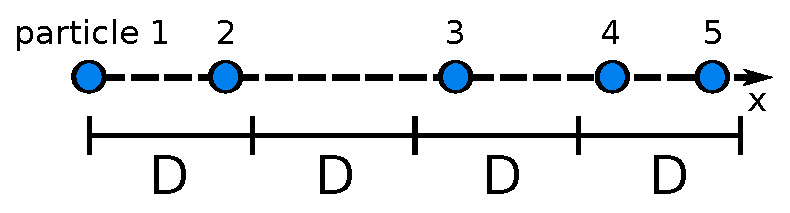
\includegraphics[width=0.5\textwidth]{Figures/1Dparacrystal}
\end{center}
\caption{Schematic representation of a 1D paracrystal in real space (side view). $D$ is the average spacing between the particles.}
\label{fig:1dpara}
\end{figure}

Using the procedure described in Section~\ref{sec:partlayout}, the interference function of a one-dimensional paracrystal is given by

\begin{align*}
S_{\mathrm{1DParaCrystal}}(q_{\parallel}) &=\Re \left(\frac{1+\Phi(q_{\parallel}) }{1 - \Phi(q_{\parallel})} \right), \\
\mathrm{where}\quad \Phi(q_{\parallel}) &= \left\{
\begin{array}{c l}     
    P(q_{\parallel}) & \mathrm{if\ \Code{corr\_length}}=0\\
    P(q_{\parallel})\exp\left(-\frac{D}{\mathrm{\Code{corr\_length}}}\right) & \mathrm{otherwise}
\end{array}\right.&
\end{align*}
%$\kappa$  is the size-distance coupling constant (equal to 0 by default) for Size Spacing Correlation Approximation

\paragraph{Example}
To illustrate the 1D paracrystal interference function, we use the same sample as in the case without interference: half-spheres deposited on a substrate.

\begin{lstlisting}[language=python, style=eclipseboxed,numbers=none,nolol,caption={\Code{Python} script to define the 1D paracrystal interference function between half-spheres, where \Code{trsphere} is of type \Code{Particle}.},label={lst:1dpara}]
    particle_layout = ParticleLayout()
    particle_layout.addParticle(trsphere, 0.0, 1.0)
    interference = InterferenceFunction1DParaCrystal(25.0*nanometer, 7*nanometer, 1e3*nanometer)
    particle_layout.addInterferenceFunction(interference)
\end{lstlisting}

\begin{figure}[h]
\begin{center}
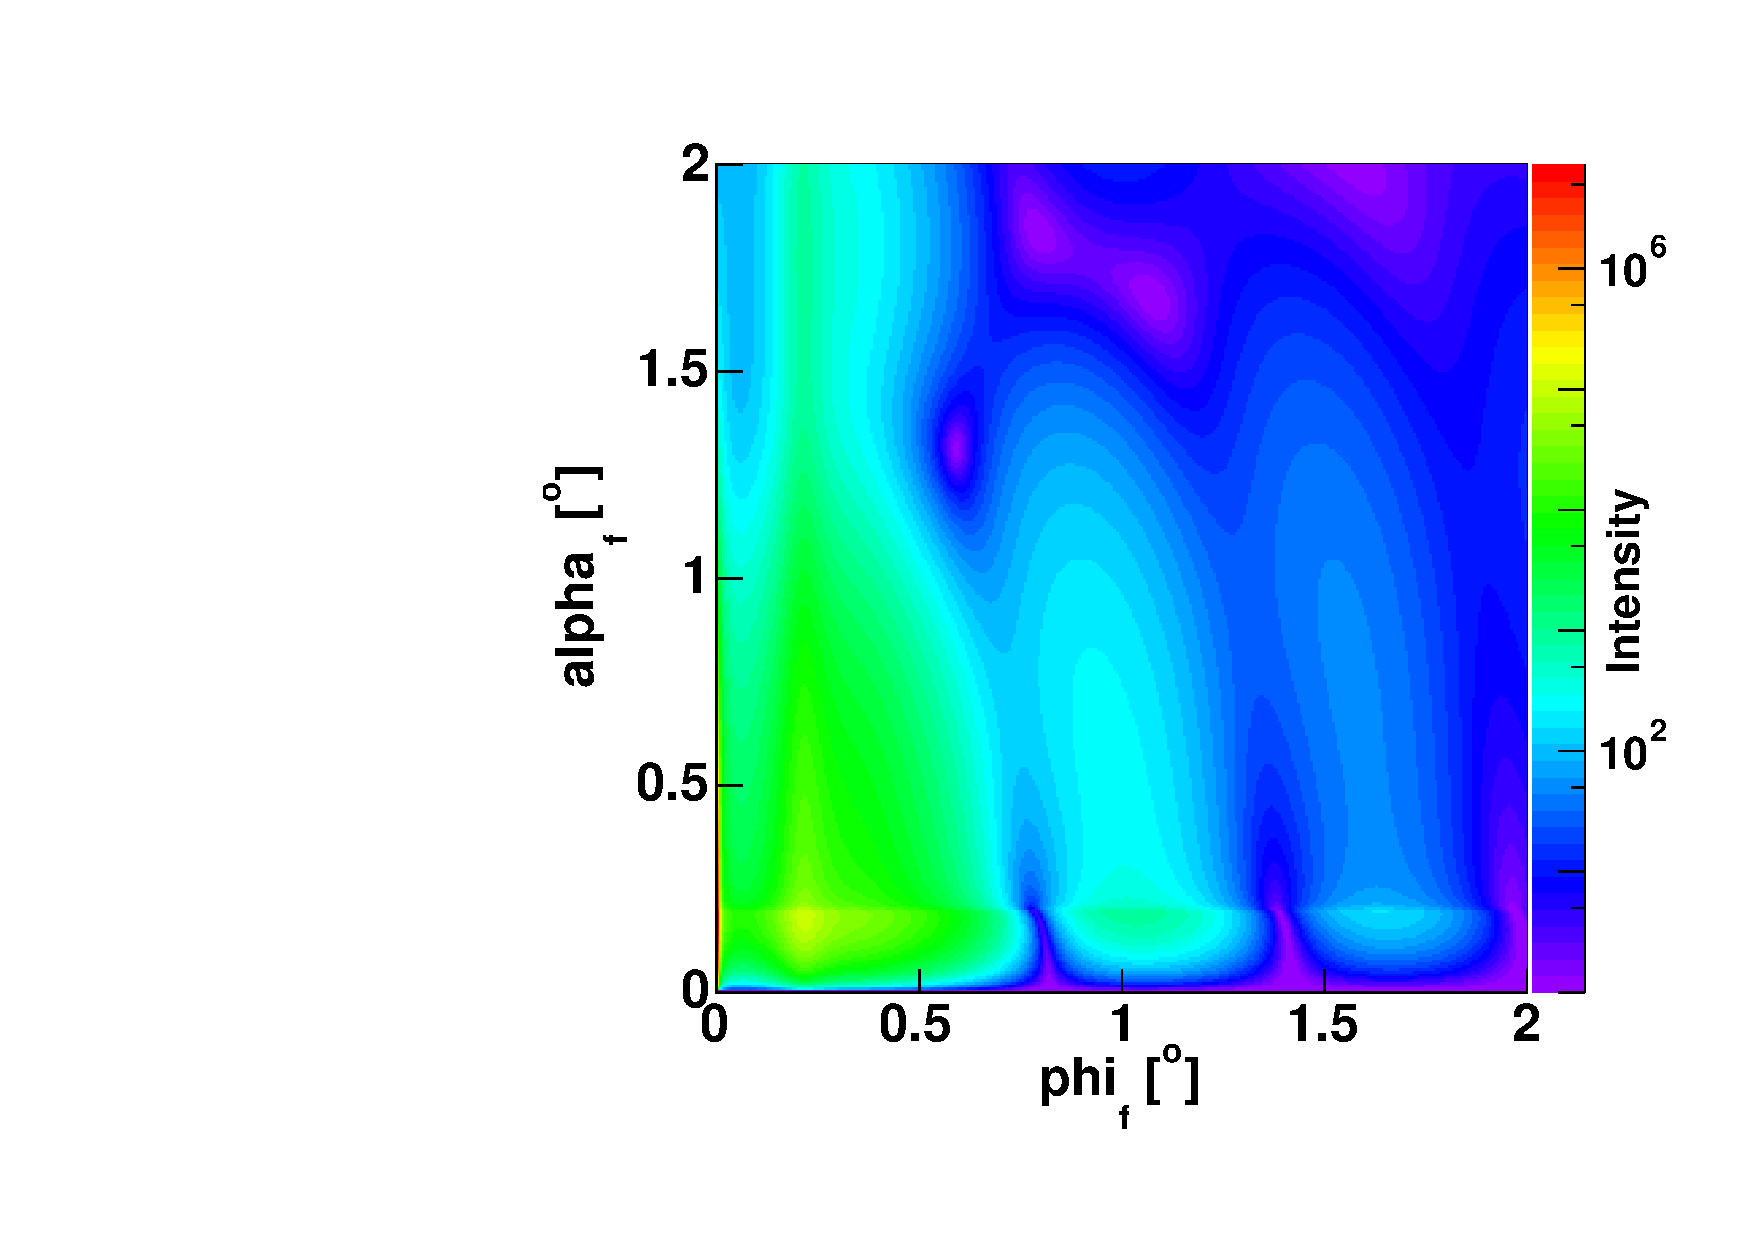
\includegraphics[width=0.5\textwidth]{Figures/HSphere_1DDL}
\end{center}
\caption{Output intensity scattered from a sample made of half-spheres with 1Dparacrystal interference between them. This figure has been generated using Script~\ref{lst:1dpara} for the interference function. The full script UMInterferences1DParaCrystal.py can be found in /Examples/python/UserManual.}
\label{fig:1ddl}
\end{figure}

\FloatBarrier

\newpage{\cleardoublepage}
%%%%%%%%%%%%%%%%%%%%%%%%%%%%%%%%%%%%%%
\subsubsection{\ding{253}  \Code{InterferenceFunction2DLattice(lattice\_parameters)}} 
where \Code{lattice\_parameters} corresponds to ($L_1$, $L_2$, $\alpha$, $\xi$)  (see illustration in figure~\ref{fig:2dlattice}) with 
\begin{itemize}
\item[]$L_1$, $L_2$ the lengths of the lattice cell, 
\item[]$\alpha$ the angle between the lattice basis vectors $\mathbf{a}, \mathbf{b}$ in direct space,
\item[] $\xi$ is the angle defining the lattice orientation (set to $0$ by default); it is taken as the angle between the $\mathbf{a}$ vector of the lattice basis and the $\mathbf{x}$ axis of the "GISAS experiment" referential (as shown in figure~\ref{fig:multil3d}).
\end{itemize}

\begin{figure}[h]
\begin{center}
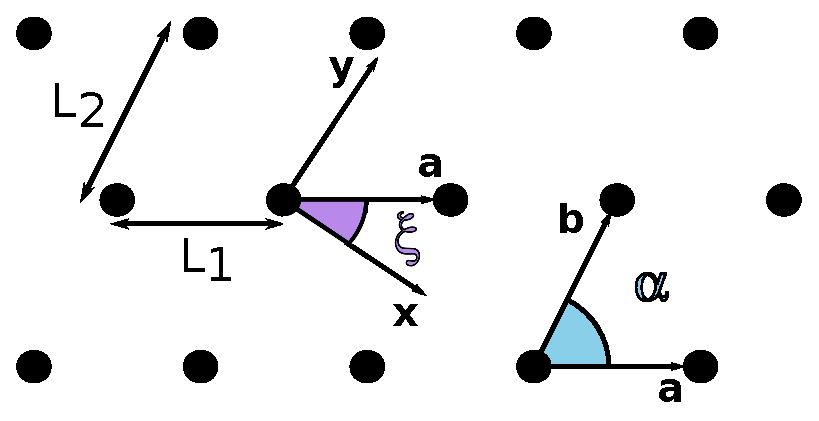
\includegraphics[width=0.5\textwidth]{Figures/2Dlattice.eps}
\end{center}
\caption{Schematic representation of a 2D lattice (top view). Such a lattice is characterized by lattice lengths $L_1$, $L_2$ and angles $\alpha$ and $\xi$.}
\label{fig:2dlattice}
\end{figure}

Like for the one-dimensional case, a probability distribution function \Code{pdf} has to be defined. One can choose between those listed in Section~\ref{baftd} and implements it using \Code{setProbabilityDistribution(pdf)}.

\paragraph{Example} The sample used to run the simulation is made of half-spheres deposited on a substrate. The interference function is "2Dlattice" and the particles are located at the nodes of a square lattice with $L_1=L_2=20$~nm, $\mathbf{a}\equiv \mathbf{b}$ and the probability distribution function is Gaussian. We also use the Local Monodisperse Approximation. 

\begin{lstlisting}[language=python, style=eclipseboxed,numbers=none,nolol,caption={\Code{Python} script to define a 2DLattice interference function between hemi-spherical particles as well as the Local Monodisperse Approximation in \Code{getSimulation()}.  The part specific to the interferences is marked in red italic font.},label={lst:2dlatticeinterf}]
    # lattice parameters
    |lattice_params = Lattice2DIFParameters()|
    |lattice_params.m_length_1 = 20.0*nanometer|
    |lattice_params.m_length_2 = 20.0*nanometer|
    |lattice_params.m_angle = 90.0*degree|
    |lattice_params.m_xi = 0.0*degree|

    #collection of particles
    sphere_ff = FormFactorTruncatedSphere(5*nanometer, 5*nanometer)
    sphere = Particle(m_particle, sphere_ff)
    |interference = InterferenceFunction2DLattice(lattice_params)|
    |pdf = FTDistribution2DGauss(200.0*nanometer/2.0/M_PI, 75.0*nanometer/2.0/M_PI)|
    |interference.setProbabilityDistribution(pdf)|
    particle_layout = ParticleLayout()
    particle_layout.addParticle(sphere, 0.0, 1.0)
    |particle_layout.addInterferenceFunction(interference)|
\end{lstlisting}
 
\begin{lstlisting}[language=python, style=eclipseboxed,numbers=none,nolol]
def get_simulation():
    """
    Create and return GISAXS simulation with beam and detector
    """
    simulation = Simulation()
    simulation.setDetectorParameters(100, 0.0*degree, 2.0*degree, 100, 0.0*degree, 2.0*degree, True)
    simulation.setBeamParameters(1.0*angstrom, 0.2*degree, 0.0*degree)
    |sim_params= SimulationParameters()|
    |sim_params.me_if_approx = SimulationParameters.LMA|
    |simulation.setSimulationParameters(sim_params)|
    return simulation
\end{lstlisting}


\begin{figure}[h]
\begin{center}
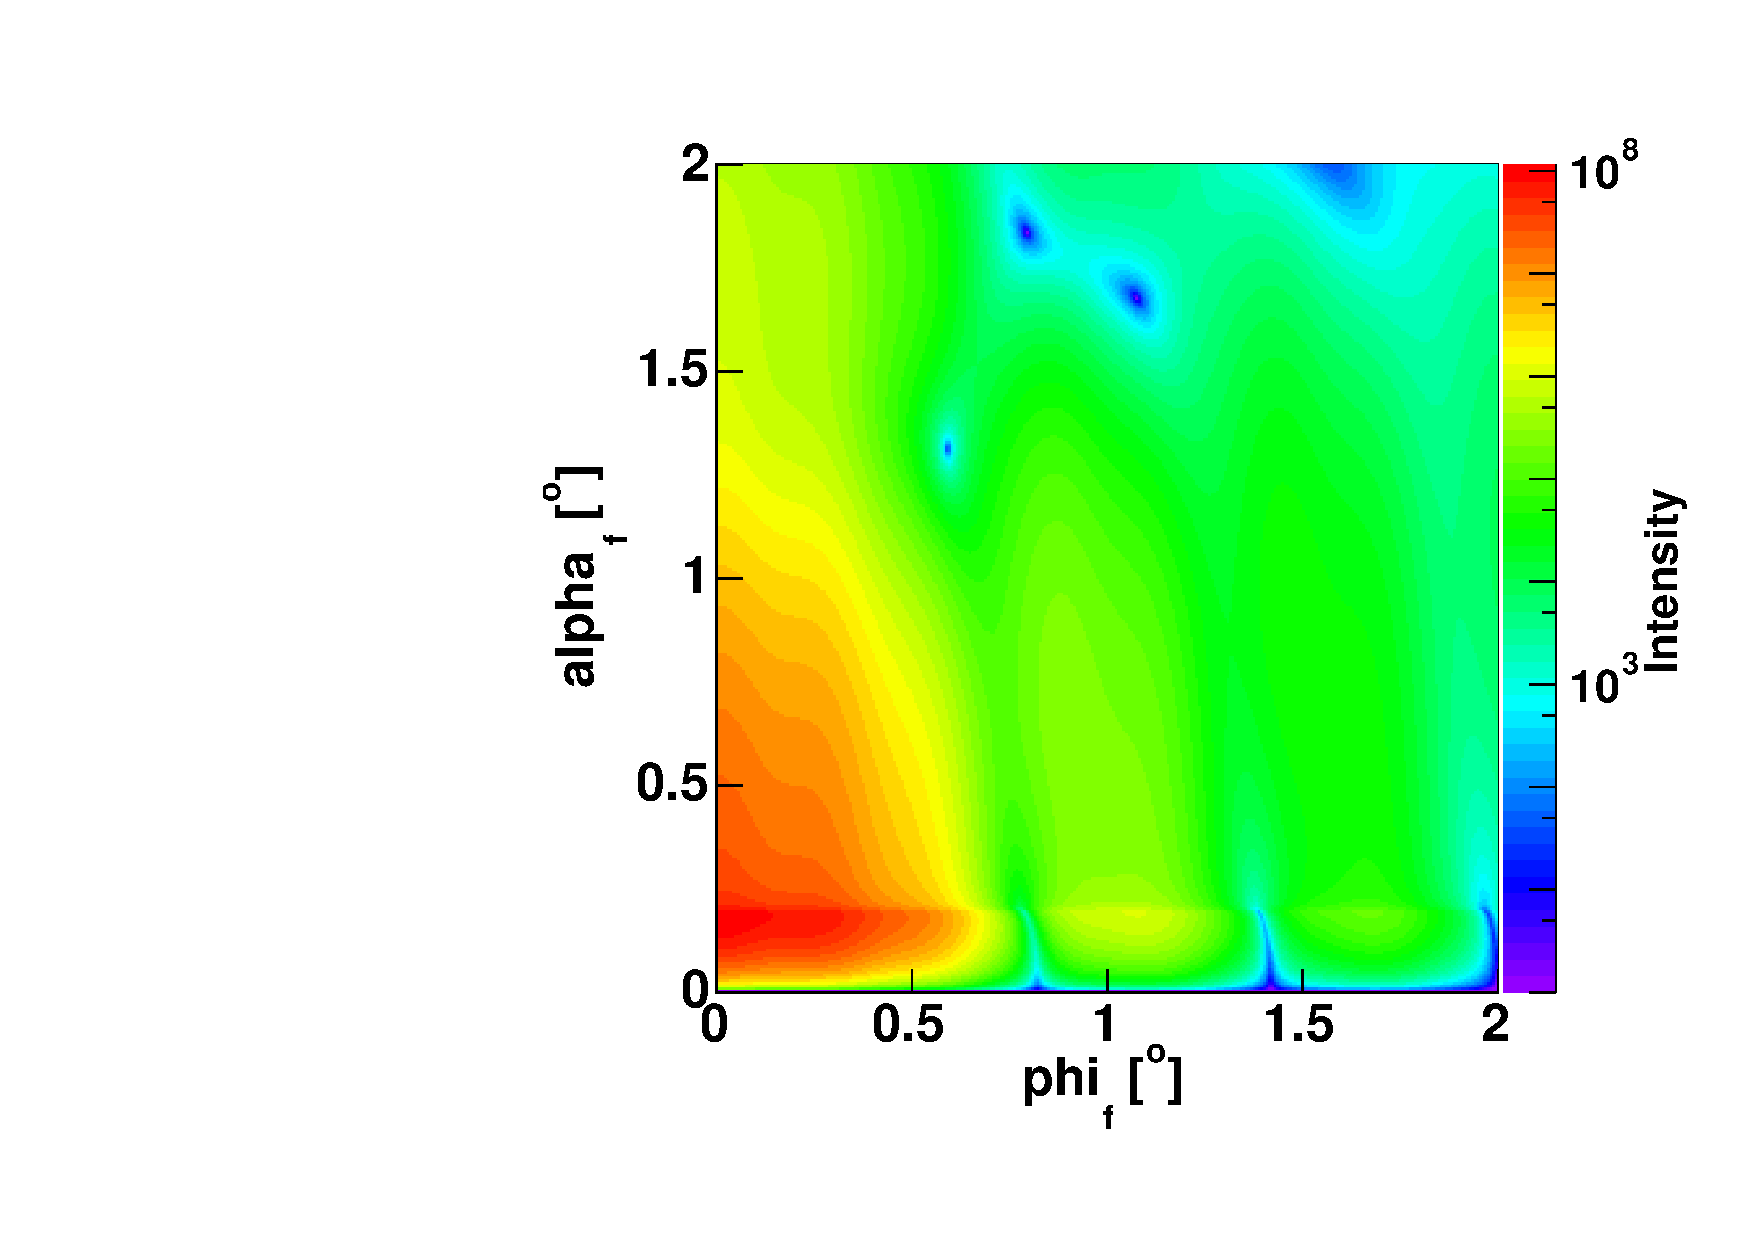
\includegraphics[width=0.5\textwidth]{Figures/HSphere_2Dlattice}
\end{center}
\caption{Output intensity scattered from a sample made of half-spheres with 2DLattice interference function. \Python\ script available in {/Examples/python/UserManual/UMInterferences2DLattice.py}.}
\label{fig:2dlatticeintensity}
\end{figure}

\FloatBarrier

\newpage{\cleardoublepage}
%%%%%%%%%%%%%%%%%%%%%%%%%%%%%%%%%%%%%%%
\subsubsection{\ding{253} \Code{InterferenceFunction2DParaCrystal(L\_1, L\_2, lattice\_angle, $\xi$, damping\_length)}} 
\begin{itemize}
\item[where] $L_1$, $L_2$ are the lengths of the lattice cell,
\item[] lattice\_angle the angle between the lattice basis vectors $\mathbf{a}, \mathbf{b}$ in direct space,
\item[] $\xi$ is the angle defining the lattice orientation (set to $0$ by default).
\item[] \Code{damping\_length} is a "damping" length. It is used to introduce finite size effects by applying a multiplicative coefficient equal to  $\exp$(\Code{peak\_distance/damping\_length}) to the Fourier transform of the probability densities. It is equal to 0 by default and, in this case, no correction is applied.
\end{itemize}
Two predefined interference functions can also be used:
\begin{itemize}
\item  \Code{createSquare(peak\_distance, damping\_length, domain\_size\_1, domain\_size\_2)}\\
where the angle between the base vectors of the lattice is set to $\pi/2$,
it creates a squared lattice,
\item \Code{createHexagonal(peak\_distance, damping\_length, domain\_size\_1, domain\_size\_2)}\\
where the angle between the base vectors of the lattice is set to $2\pi/3$ ,
\end{itemize}
where
\Code{domain\_size1, 2} are the dimensions of coherent domains of the paracrystal along the main axes,\\ \Code{peak\_distance} is the same in both directions and $\mathbf{a}\equiv \mathbf{x}$.\\

Probability distribution functions have to be defined. As the two-dimensional paracrystal is defined from two independent 1D paracrystals, we need two of these functions, using\\ \Code{setProbabilityDistributions(pdf\_1, pdf\_2)}, with \Code{pdf\_{1,2}} are related to each main axis of the paracrystal.


\paragraph{Example} The particles deposited on a substrate are half-spheres. They interference via the 2DParacrystal distribution function. The paracrystal is based on a 2D hexagonal lattice with a Gaussian probability distribution function in reciprocal space.  Script~\ref{lst:2dlatticeinterf} shows the implementation of the interference function and fig.~\ref{fig:2ddl} an example of output intensity using hemi-spherical particles The full script, UMInterferences2DParacrystal.py is available in /Examples/python/UserManual.

\begin{lstlisting}[language=python, style=eclipseboxed,numbers=none,nolol,caption={\Code{Python} script to define a "2DParacrystal" interference function between particles forming an hexagonal monolayer. },label={lst:2dlatticeinterf}]
    interference = InterferenceFunction2DParaCrystal.createHexagonal(30.0*nanometer,0.0, 40.0*micrometer, 40.0*micrometer)|
    pdf = FTDistribution2DCauchy(1.0*nanometer, 1.0*nanometer)
    interference.setProbabilityDistributions(pdf, pdf)
    particle_decoration.addInterferenceFunction(interference)
\end{lstlisting}

\begin{figure}[h]
\begin{center}
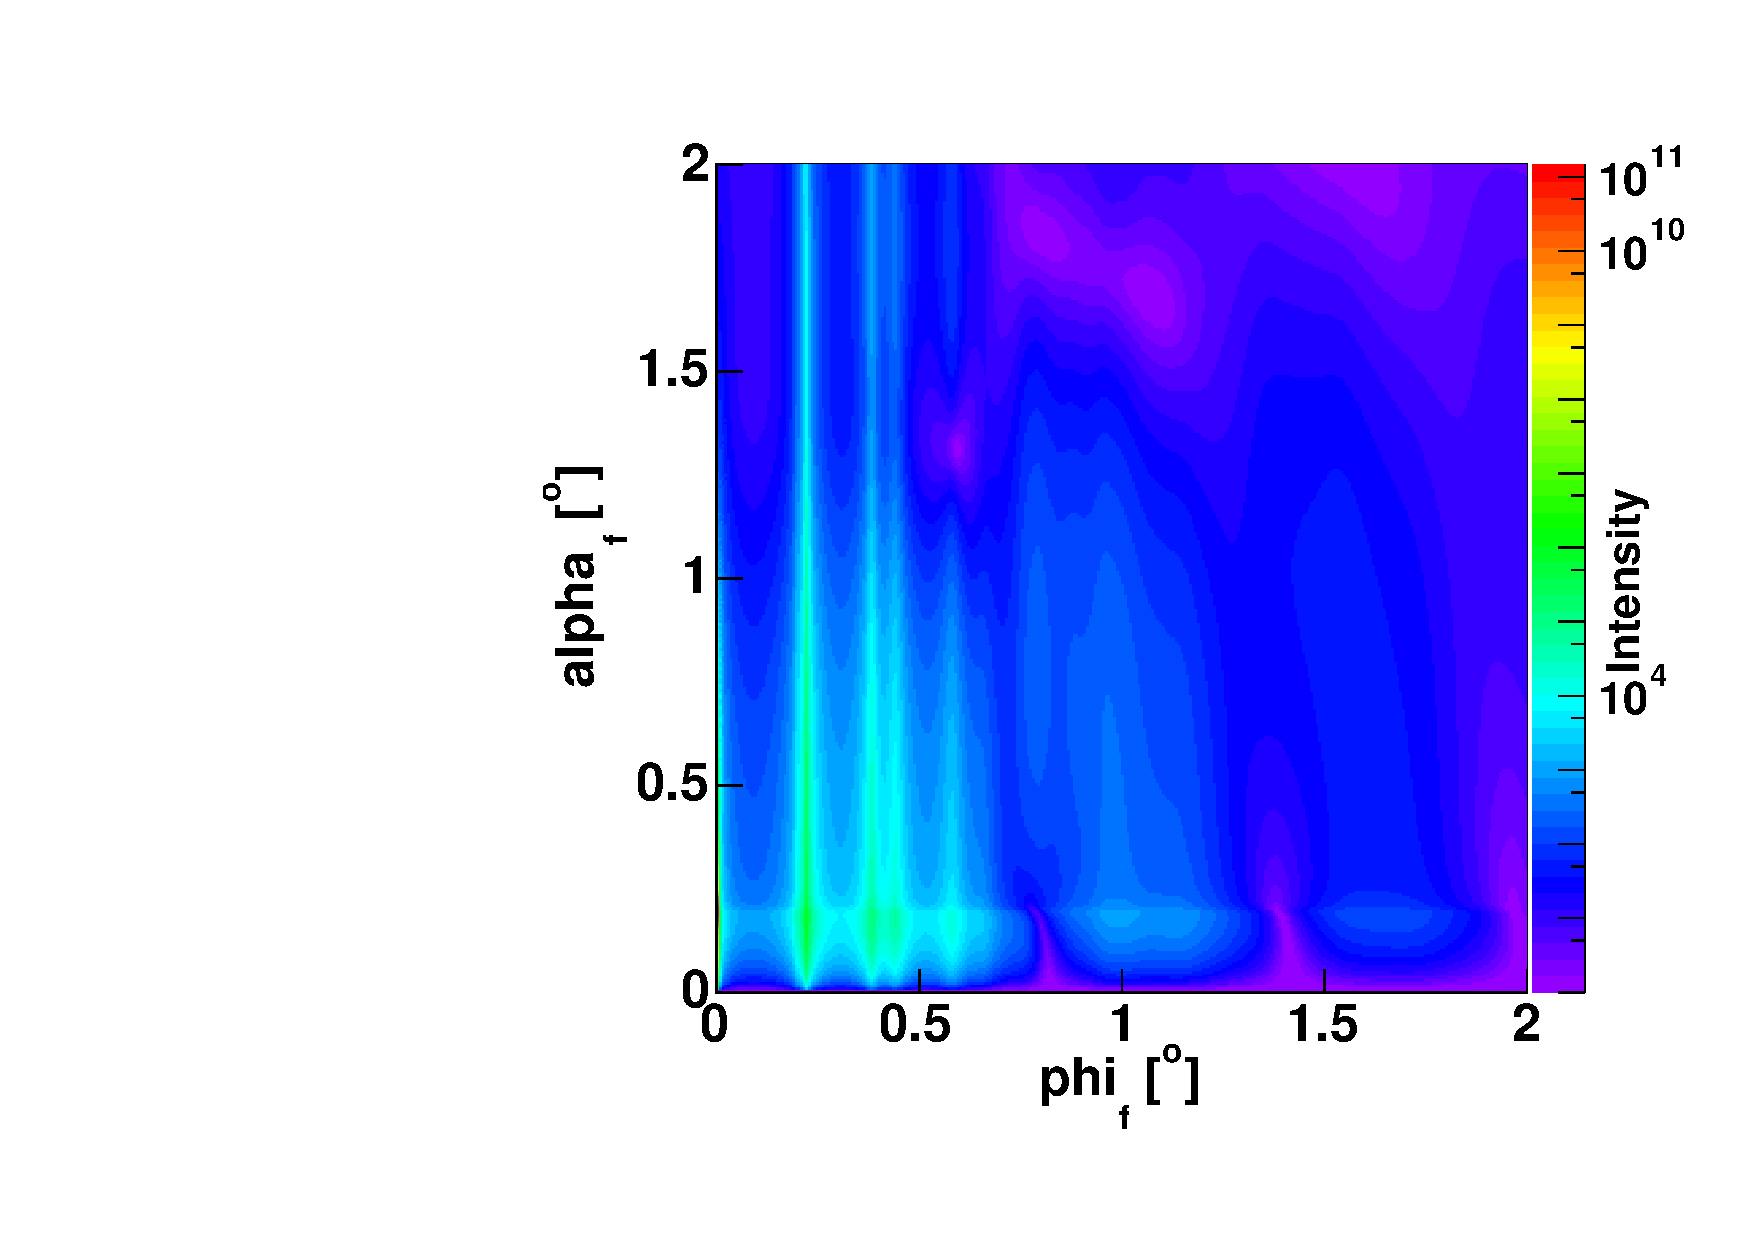
\includegraphics[width=0.5\textwidth]{Figures/HSphere_2DDL}
\end{center}
\caption{Output intensity scattered from a sample made of half-spheres with 2DParacrystal interference function.}
\label{fig:2ddl}
\end{figure}

\FloatBarrier

%%%%%%%%%%%%%%%%%%%%%%%%%%%%%%%%%%%%%%%%
\subsection{Summary}

\begin{landscape}
\begin{table}
\begin{tabular}{lll}
\hline
Function  & Parameters & Comments\\
\hline
\Code{InterferenceFunctionNone}  & None & disordered distribution \\
\hline
\Code{InterferenceFunction1DLattice} & \Code{lattice\_length} & use only with infinitely long/wide particles \\
  & $\xi=\widehat{(\mathbf{x},\mathbf{a})}$ & pdf=(Cauchy, Gauss or Voigt)  to be defined\\
\hline
 \Code{InterferenceFunction1DParaCrystal}  & peak\_distance of pdf & only Gaussian pdf implemented (no option)\\
   & width of pdf &\\
& corr\_length (optional) & \\
\hline
 \Code{InterferenceFunction2DLattice}  & L\_1, L\_2: lattice lengths & pdf=(Cauchy, Gauss or Voigt) to be defined\\
                        & lattice\_angle=$\widehat{(\mathbf{a},\mathbf{b})}$ & \\
                                                            & $\xi =\widehat{(\mathbf{x},\mathbf{a})}$ & \\                                                  
\hline
\Code{InterferenceFunction2DParaCrystal}  & L\_1, L\_2: lattice lengths & 2D pdf=(Cauchy, Gauss or Voigt) to be defined \\
                          & lattice\_angle=$\widehat{(\mathbf{a},\mathbf{b})}$ & (1 pdf per axis) \\
& $\xi=\widehat{(\mathbf{x},\mathbf{a})}$ & \\
& damping\_length (optional)  &  same for both axes\\
\hline
\hline
\end{tabular}
\caption{List of interference functions implemented in \BornAgain. pdf : probability distribution function, $\mathbf{a}, \mathbf{b}$ are the lattice base vector, and $\mathbf{x}$ is the axis vector perpendicular to the detector plane.}
\end{table}
\end{landscape}

%%%%%%%%%%%%%%%%%%%%%%%%%%%%%%%
\section{Particles - Form factors} \SecLabel{sect:ff}

\subsection{Born approximation}

In \BornAgain\ the form factor is defined using Born approximation as
\begin{equation}
F(\mathbf{q})=\int_V \exp (i\mathbf{q}.\mathbf{r}) d^3 \mathbf{r},
\label{ffformulaBA}
\end{equation}
where $V$ is the volume of the particle's shape,
$\mathbf{q}=\mathbf{k}_i - \mathbf{k}_f$ is the scattering vector with
$\mathbf{k}_f$ and $\mathbf{k}_i$ the scattered and incident wave
vector, respectively.\\

The particle's shape is parametrized in a cartesian frame, with its
$z$-axis pointing upwards and its origin at the center of the bottom
of the particle: $\mathbf{r}=(x,y,z)$. 

All form factors have been implemented with complex scattering vectors
in order to take any material absorption into account.

Table~\ref{tab:formfactors} lists the particles shapes whose form
factors have been implemented in \BornAgain\ and a detailed description is given in Appendix \ref{appendixff}.

\newpage

\begin{table}[H] 
\caption{Table of form factors implemented in \BornAgain.} \label{tab:formfactors}
  \begin{tabulary} {\textwidth}{Lc Lc L c L} 
\hline 
Box,\phantom{-} \SecRef{Box} & & Prism3,  \SecRef{Prism3} & & Tetrahedron, \SecRef{Tetrahedron} & & Prism6,  \SecRef{Prism6}\\
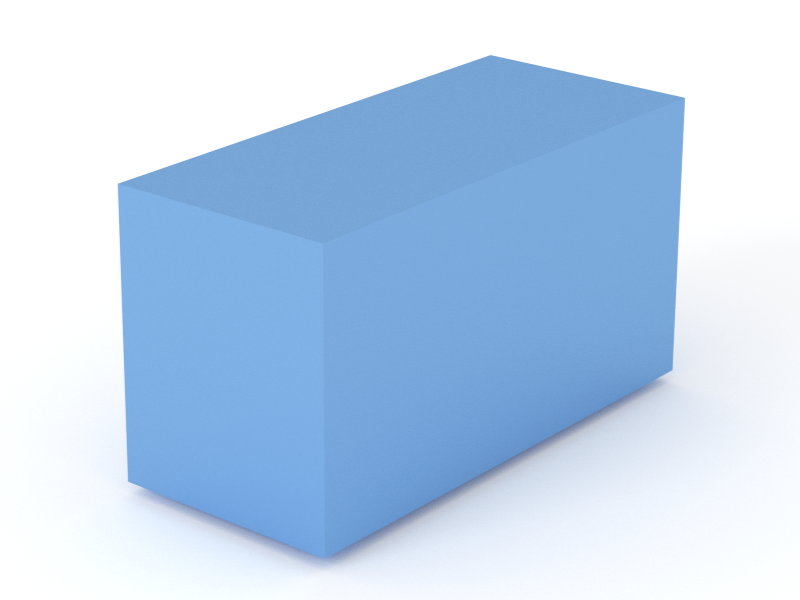
\includegraphics[width=1in]{Figures/Box3d} & & 
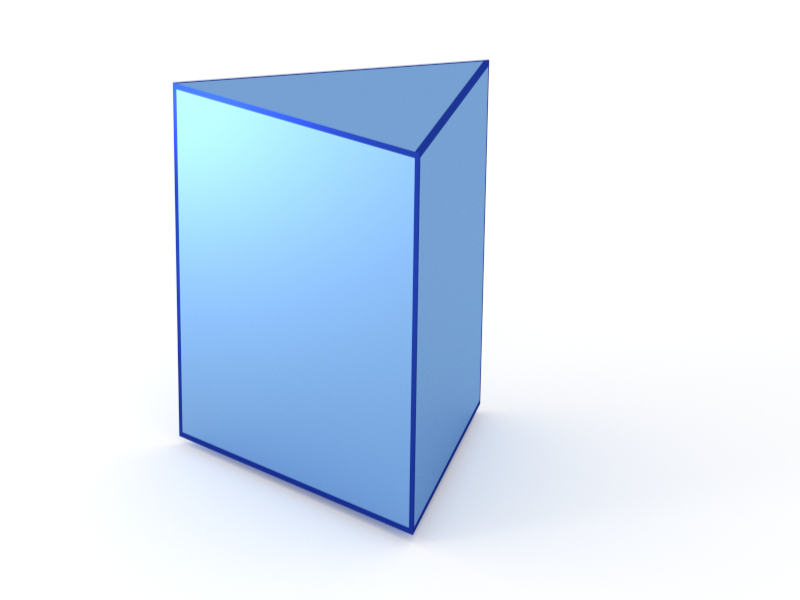
\includegraphics[width=1in]{Figures/Prism33d} & & 
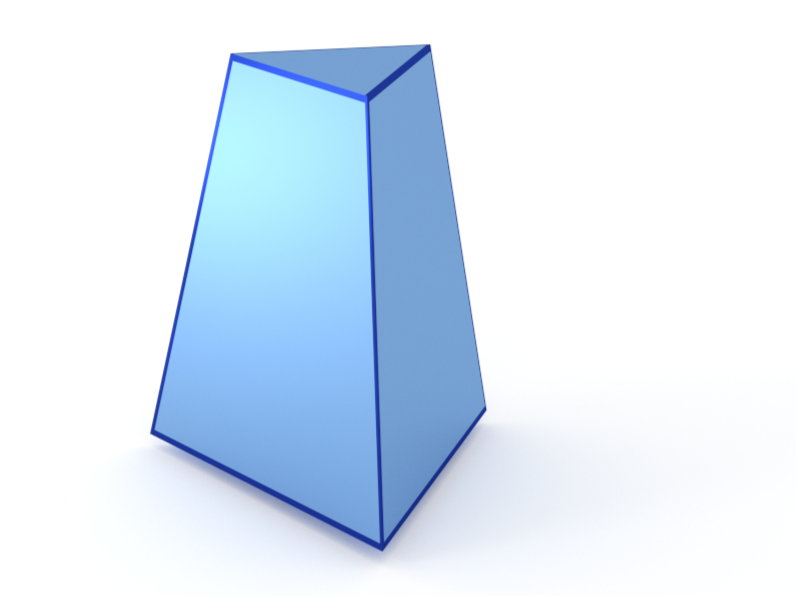
\includegraphics[width=1in]{Figures/Tetrahedron3d} & & 
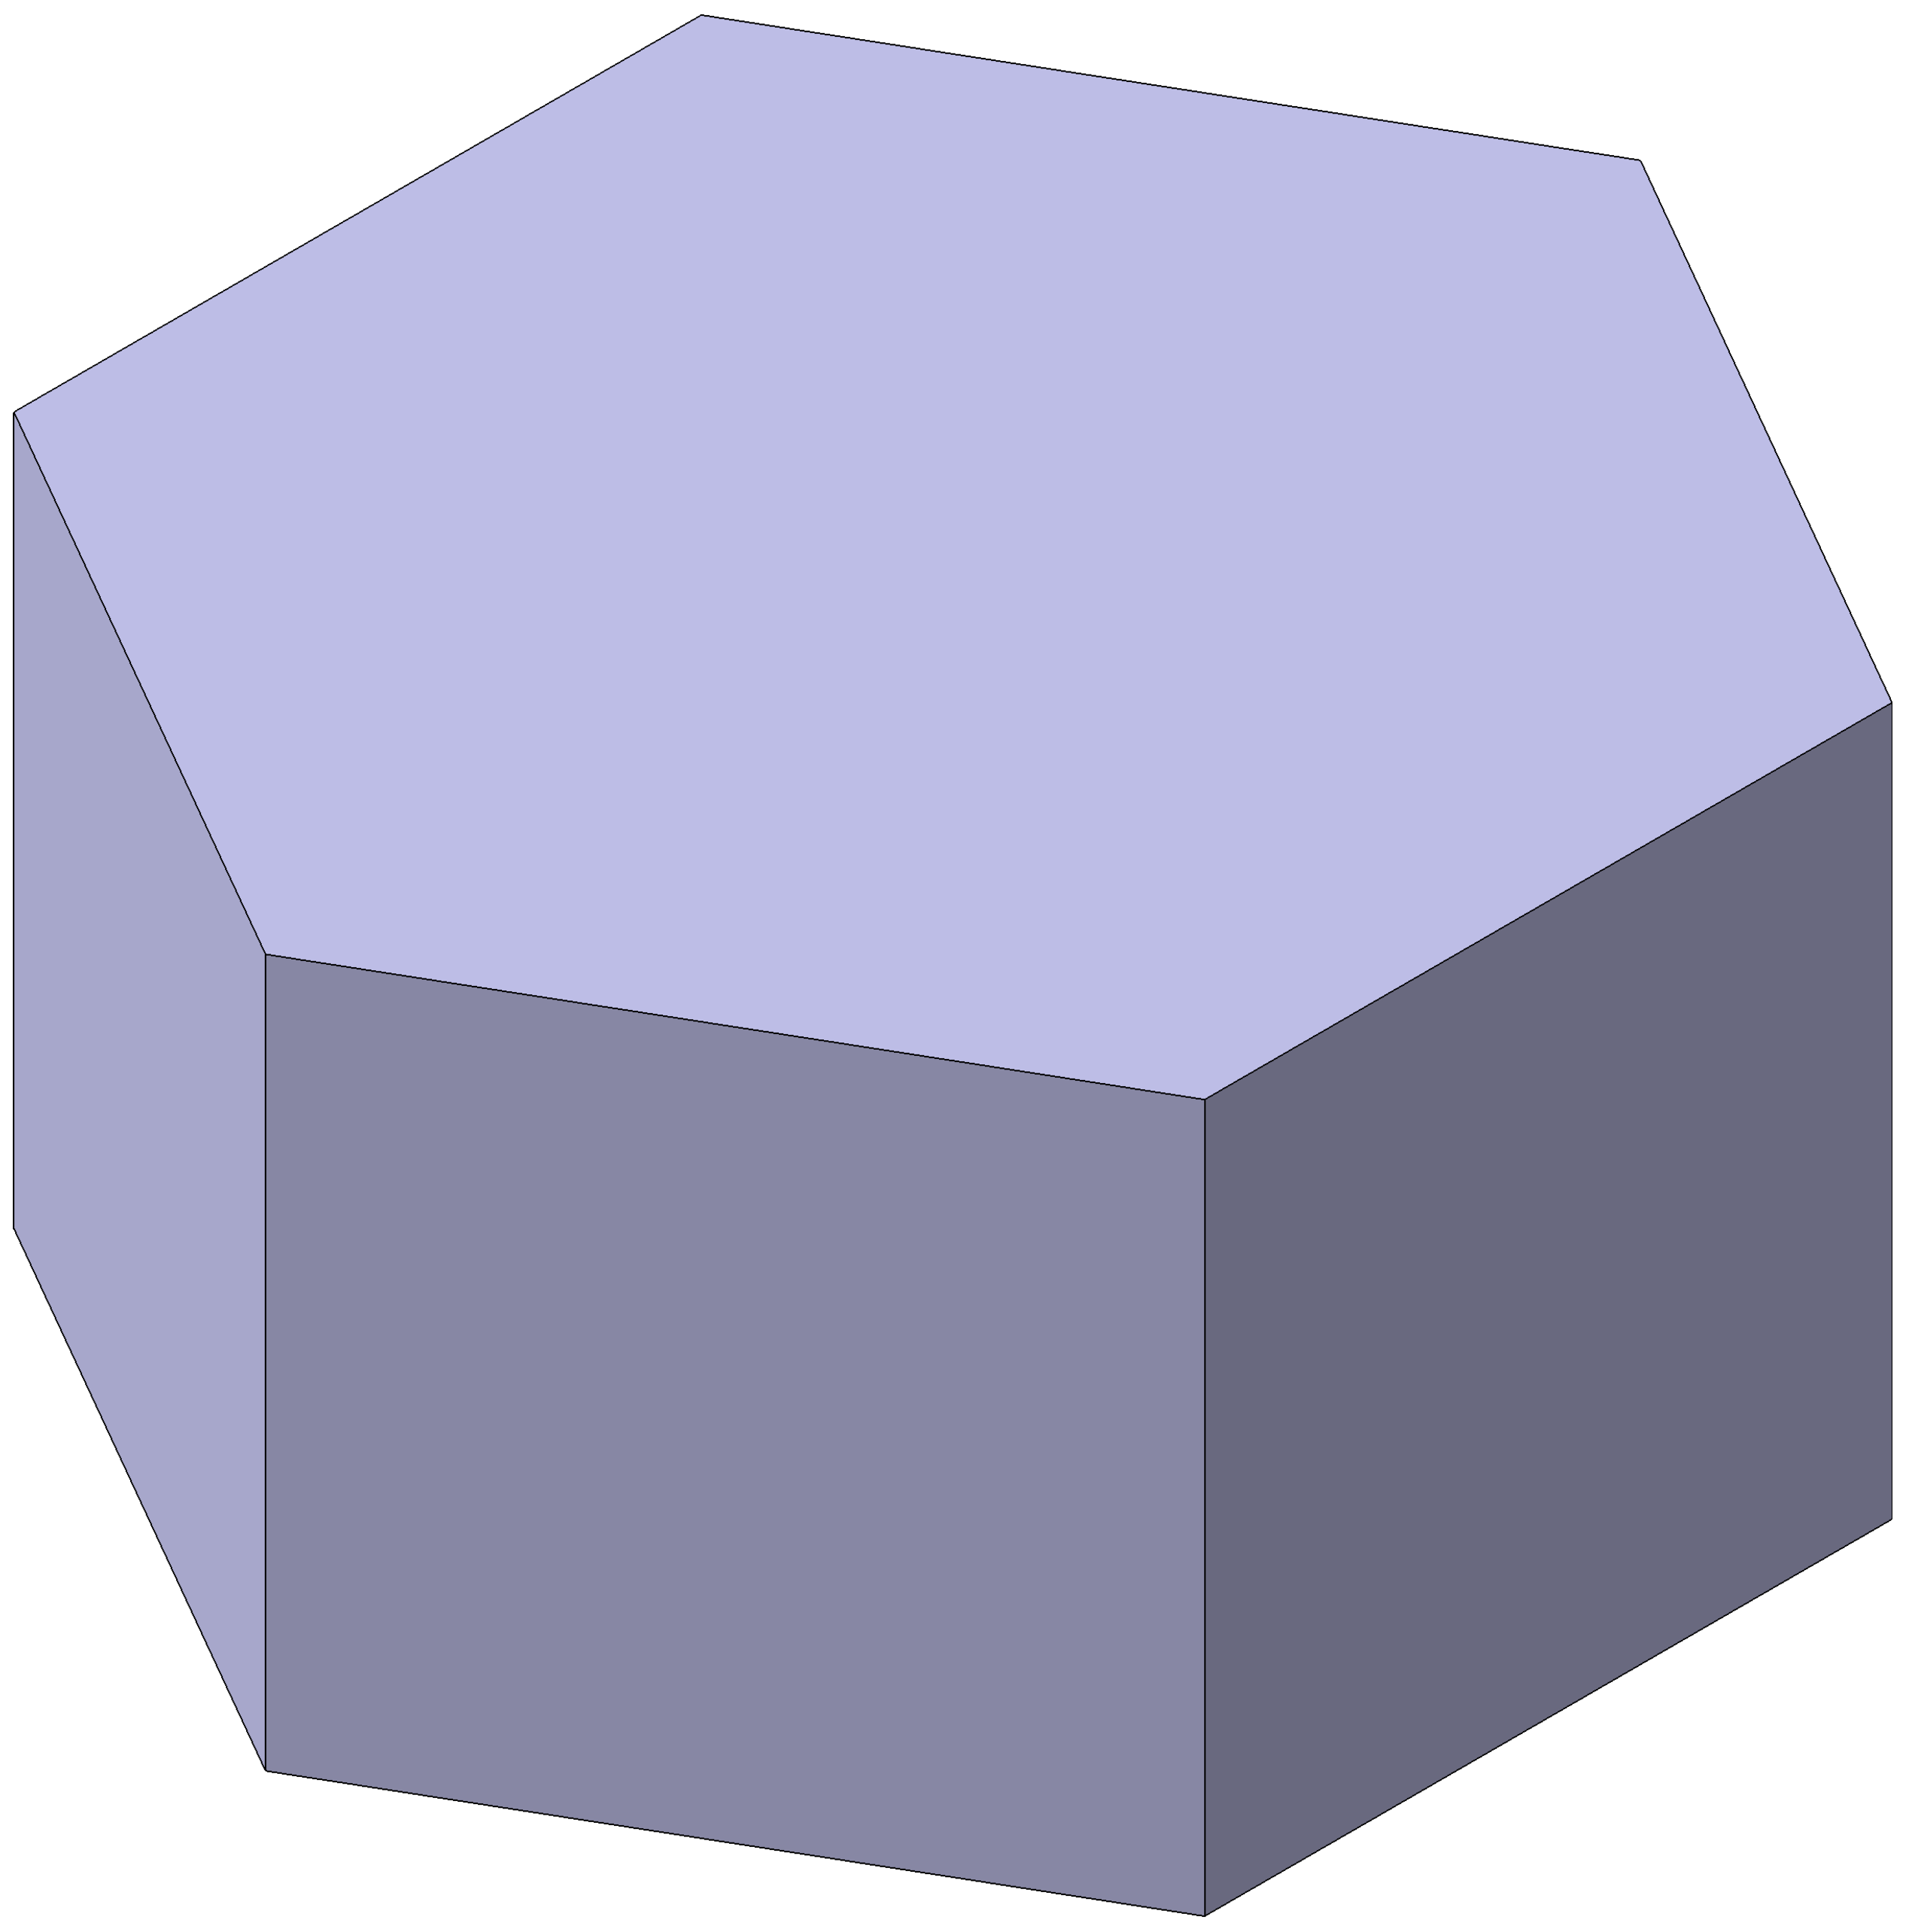
\includegraphics[width=1in]{Figures/Prism63d} 
\\
\hline 
Cone6,  \SecRef{Cone6} & &  Pyramid, \SecRef{Pyramid} & & Anisotropic pyramid,  \SecRef{AnisoPyramid} & &  {Cuboctahedron}, \SecRef{Cuboctahedron}\\
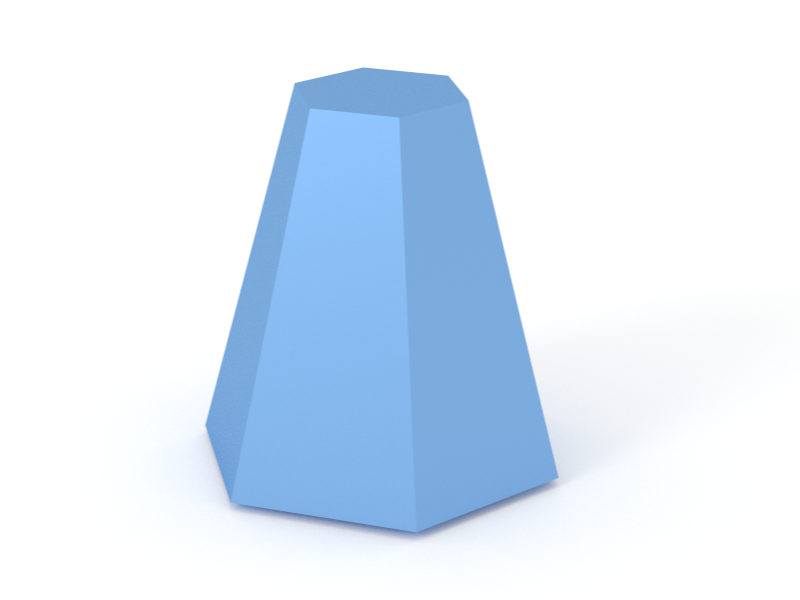
\includegraphics[width=1in]{Figures/Cone63d}  & & 
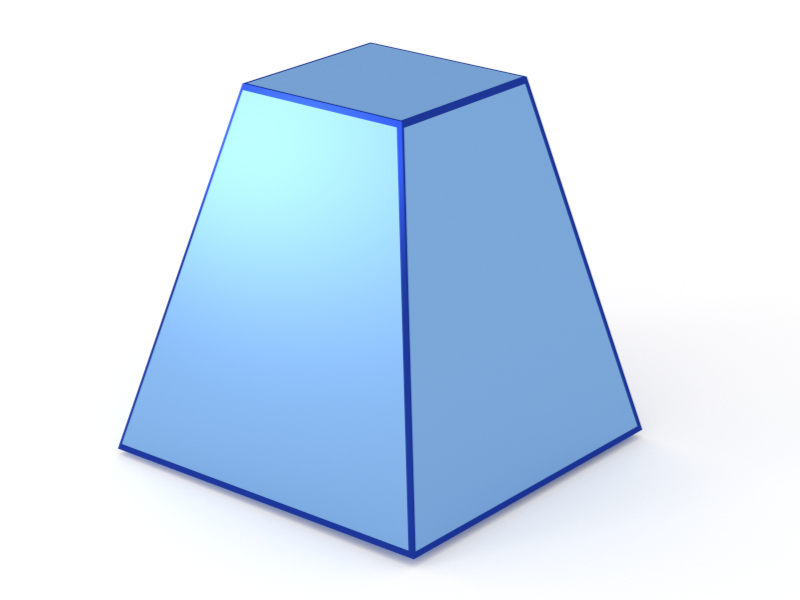
\includegraphics[width=1in]{Figures/Pyramid3d} & &
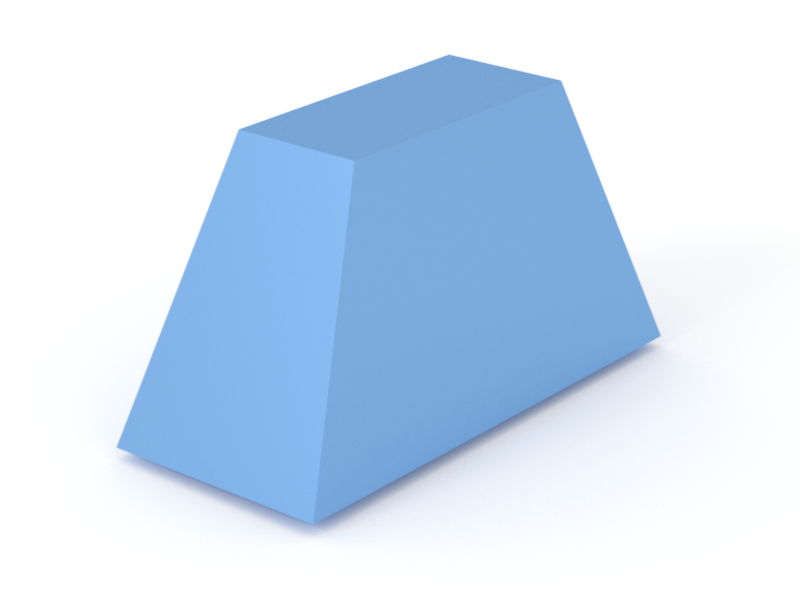
\includegraphics[width=1in]{Figures/AnistropicPyramid3d} & & 
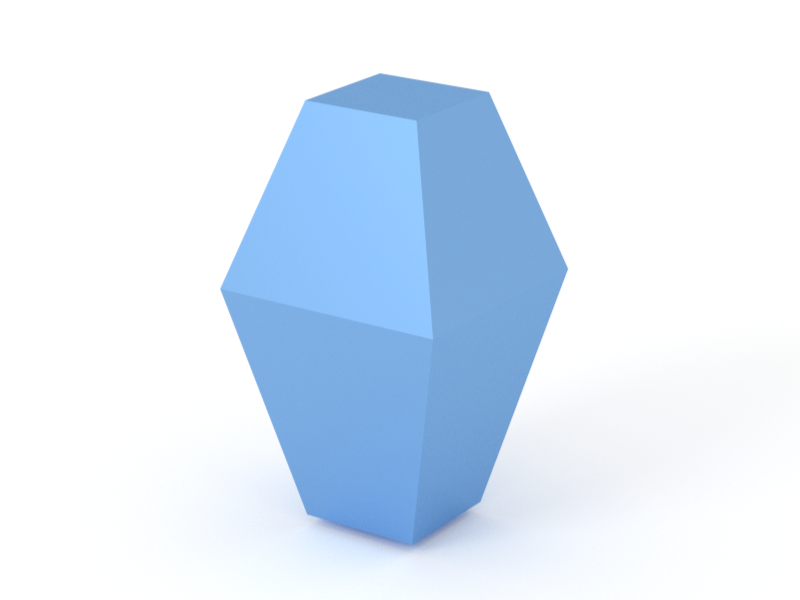
\includegraphics[width=1in]{Figures/Cuboctahedron3d}
\\
\hline
Cylinder, \SecRef{Cylinder}  & & Ellipsoidal cylinder, \SecRef{EllipsoidalCylinder} & &  Cone,\phantom{--} \SecRef{Cone} & & Full Sphere, \SecRef{FullSphere} \\
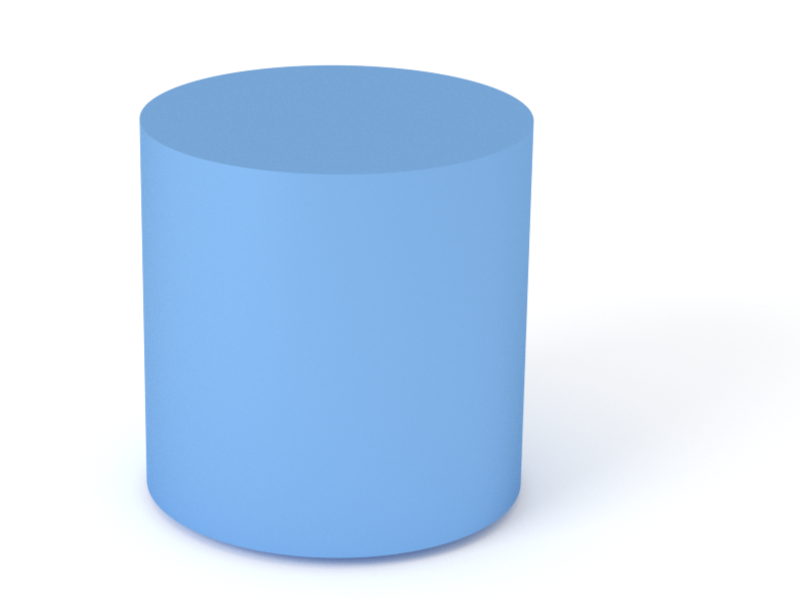
\includegraphics[width=1in]{Figures/Cylinder3d} & & 
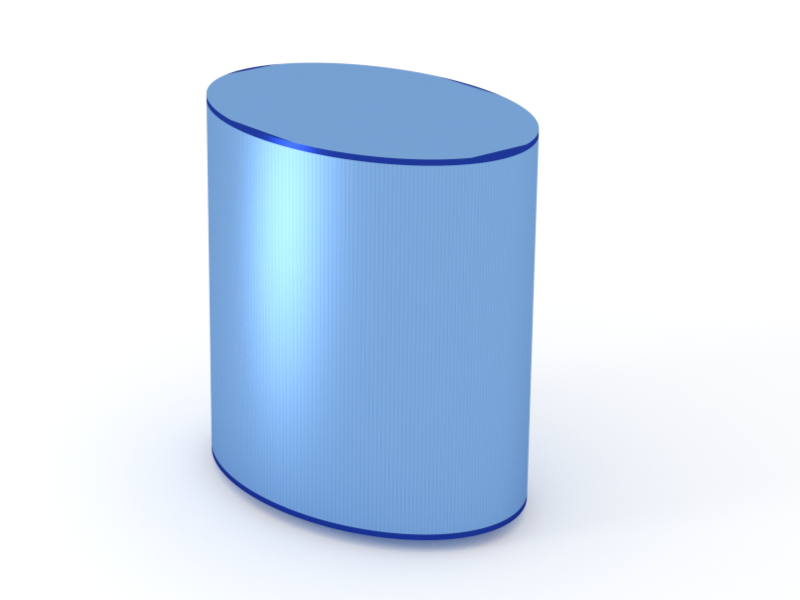
\includegraphics[width=1in]{Figures/EllipsoidalCylinder3d} & & 
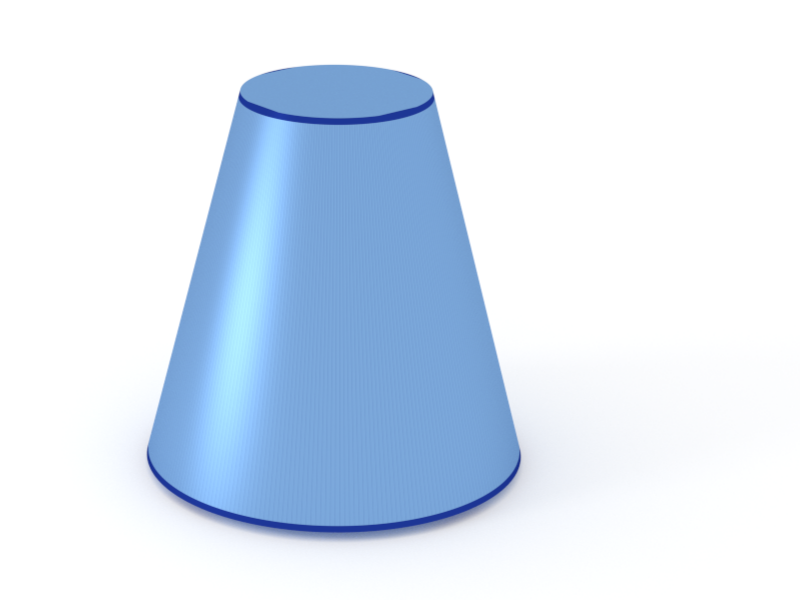
\includegraphics[width=1in]{Figures/Cone3d} & & 
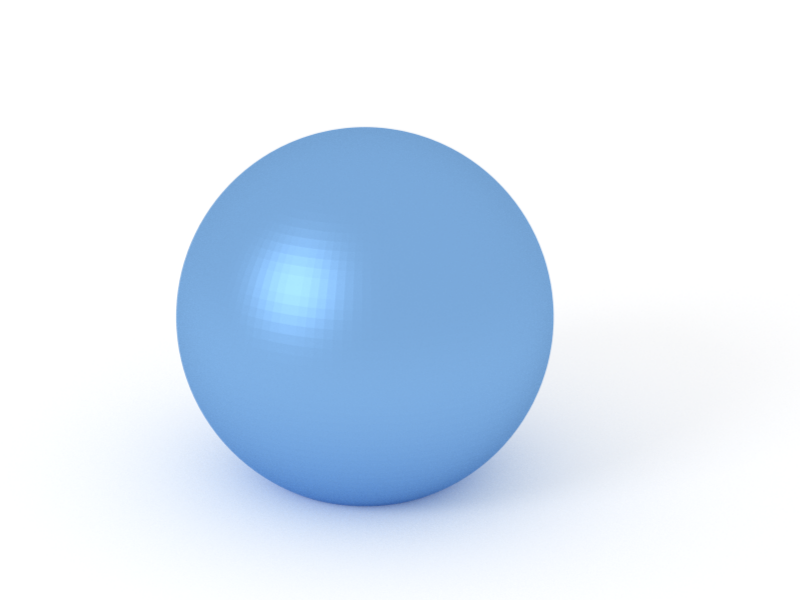
\includegraphics[width=1in]{Figures/FullSphere3d} \\
\hline
Truncated Sphere, \SecRef{Sphere}  & & Full Spheroid, \SecRef{FullSpheroid} & & Truncated Spheroid,  \SecRef{Spheroid} & & Hemi Ellipsoid, \SecRef{HemiEllipsoid}\\
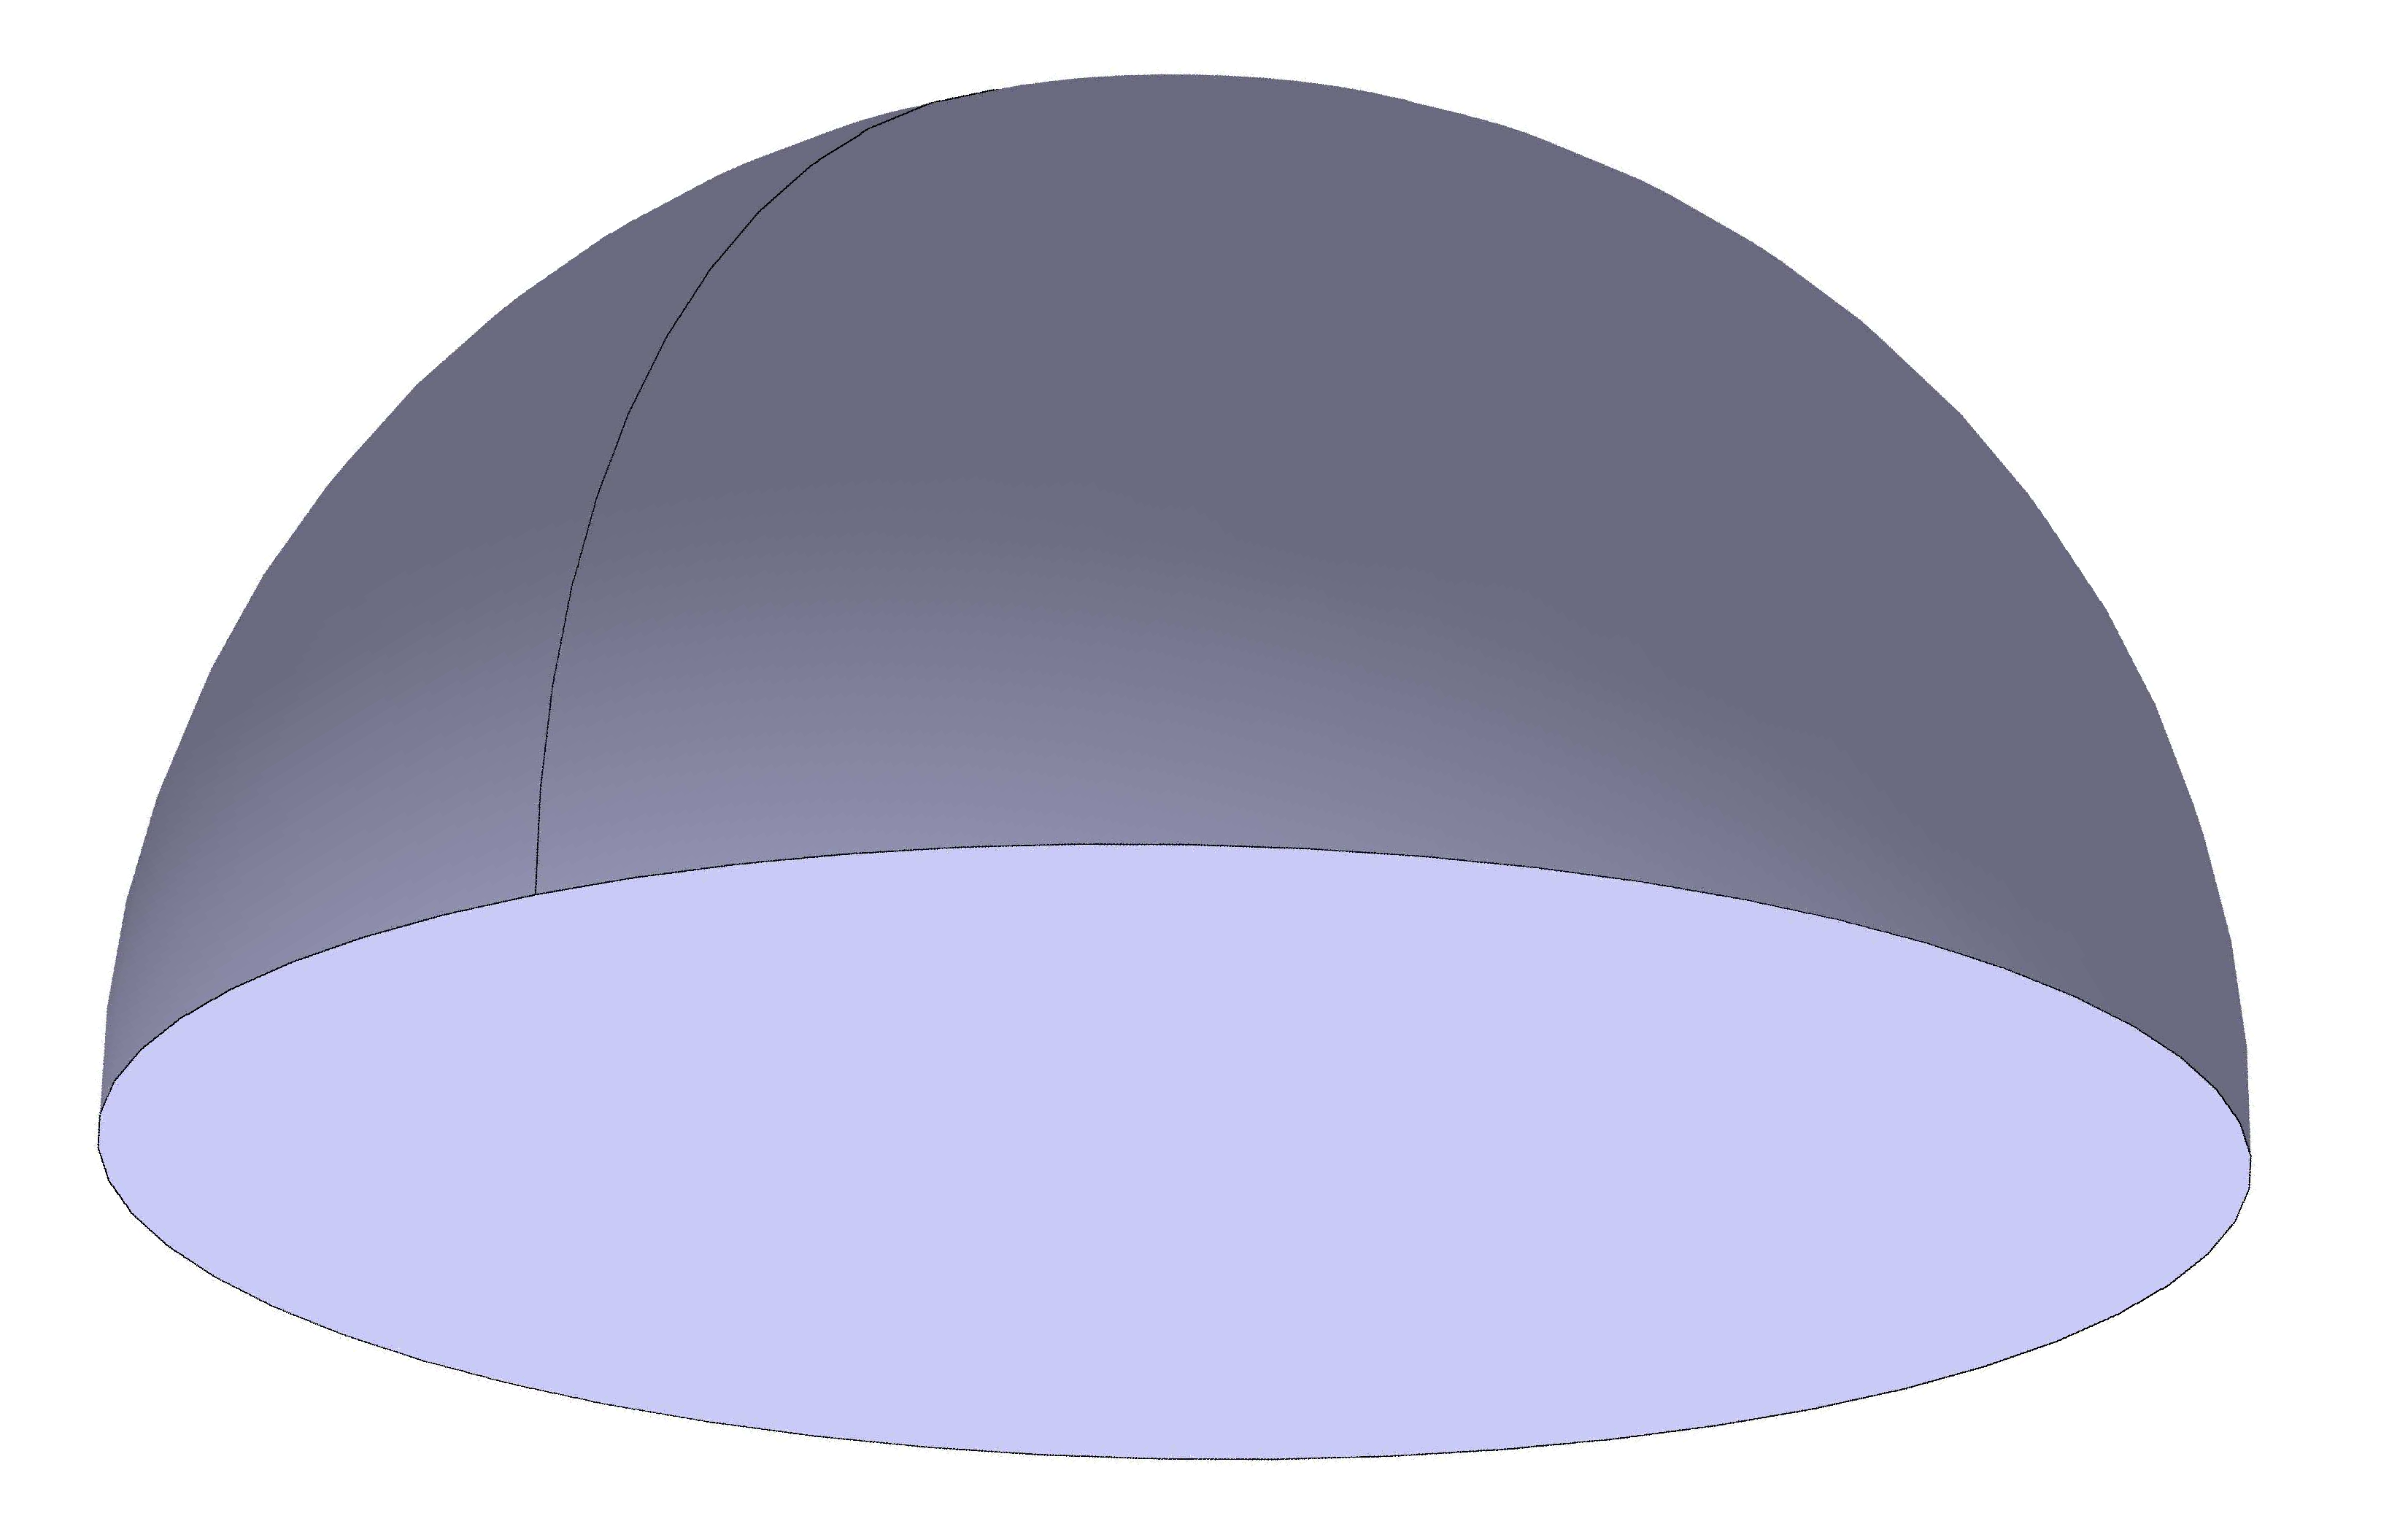
\includegraphics[width=1in]{Figures/Sphere3d}  & & 
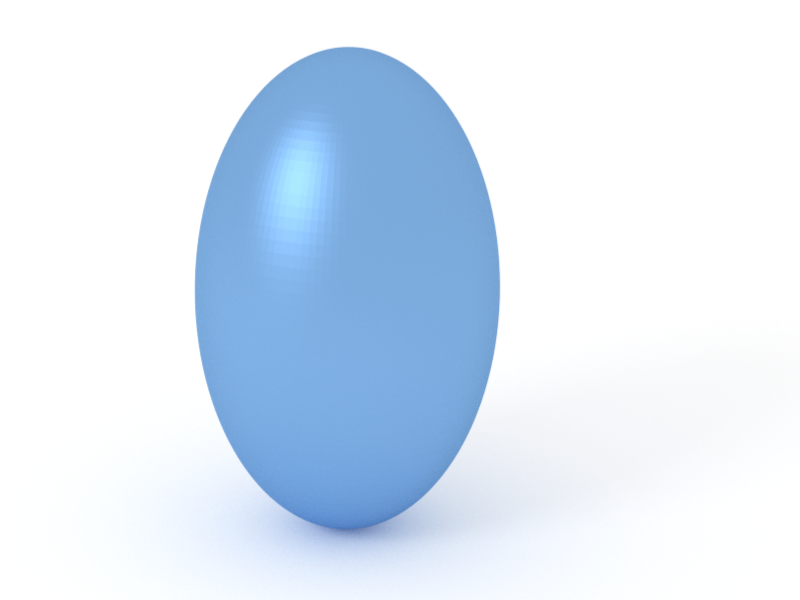
\includegraphics[width=1in]{Figures/FullSpheroid3d} & & 
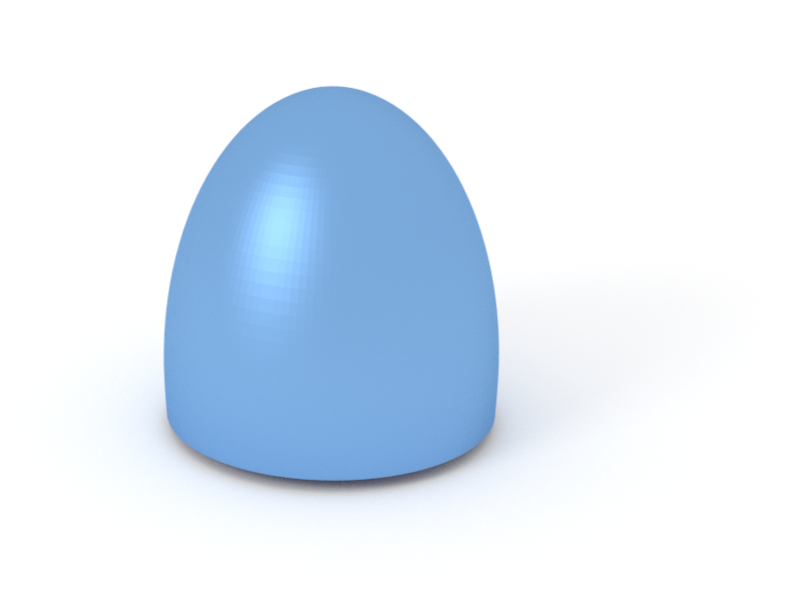
\includegraphics[width=1in]{Figures/Spheroid3d} & & 
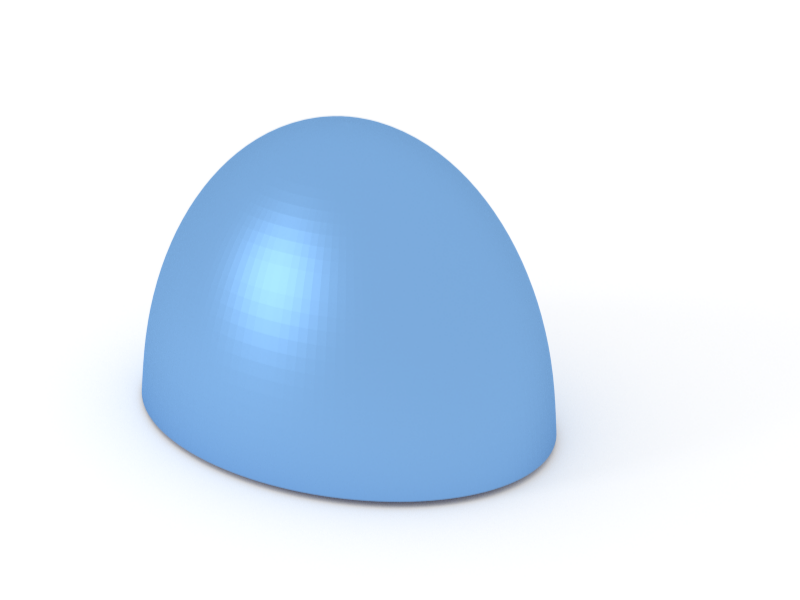
\includegraphics[width=1in]{Figures/HemiEllipsoid3d}\\
\hline
Ripple1, \SecRef{Ripple1} &  & Ripple2, \SecRef{Ripple2}& &   & &  \\
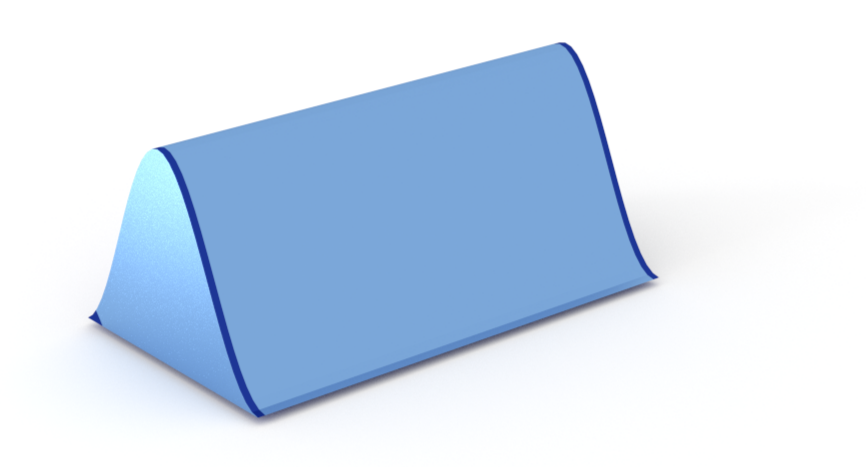
\includegraphics[width=1in]{Figures/Ripple13d} & & 
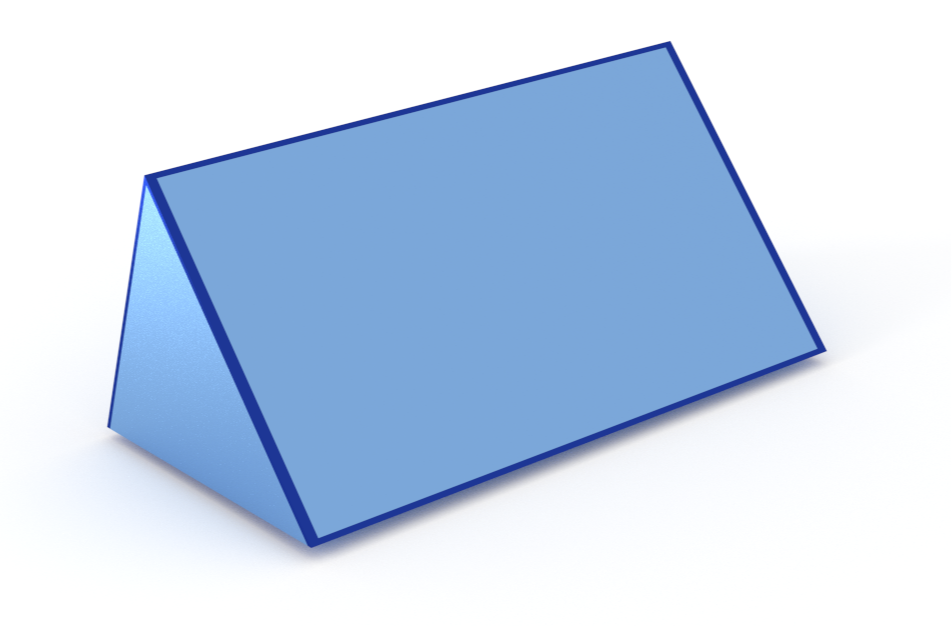
\includegraphics[width=1in]{Figures/Ripple23d} & &  & & \\
\hline 
\end{tabulary}
\end{table}

\newpage

%%%%%%%%%%%%%%%%%%%%%%%%%%%%%%%%%%%%%%%%%%%%%%%%%%%%%%%%%%%%%%%%%%%%%%%
\subsection{Distorted Wave Born Approximation} \SecLabel{sect:dwba}

Born approximation fails when multiple reflections and refractions have to be taken into account at interfaces because of the presence of underlying layers of materials and the closeness of  the incident angle $\alpha_i$ to the critical angle of total external reflection $\alpha_c$. The first order correction to the scattering theory is the Distorted Wave Born Approximation (DWBA), whereas the Born approximation is the zeroth order. \\
The collective effects between the particles are not considered in this section. They have been described in~\SecRef{sect:interf}.  We also do not take any polarization effects into account. They will be described in...\\

 In the DWBA, the form factor of a particle in a multilayer system is given by

\begin{align}
F_{\rm{DWBA}} (\vect{k}_i,\vect{k}_f, r_z) & = T_i T_f F_{\rm{BA}} (\vect{k}_i-\vect{k}_f) e^{i (k_{i,z}-k_{f,z}) r_z} + R_i T_f F_{\rm{BA}}(\vect{\widetilde{k}}_i-\vect{k}_f) e^{i(-k_{i,z}-k_{f,z})r_z}
 \nonumber \\
  &+ T_i R_f F_{\rm{BA}}(\vect{k}_i-\vect{\widetilde{k}}_f)e^{i(k_{i,z}+k_{f,z})r_z} + R_iR_fF_{\rm{BA}} (\vect{\widetilde{k}}_i-\vect{\widetilde{k}}_f)e^{i(-k_{i,z}+k_{f,z})r_z} \; , \label{eq:dwbageneral}
\end{align}
where $F_{\rm{BA}}$ is the expression of the form factor in the Born approximation, $r_z$ is the $z$-coordinate of the particle's position (measured from the bottom of the particle), $\vect{k}_i=(k_{i,x}, k_{i,y}, k_{i,z})$ $\vect{k}_f=(k_{f,x}, k_{f,y}, k_{f,z})$ are the incident and scattered wave vectors in air, respectively \cite{Raus95}. With a tilde (\~{}), these wavevectors components are evaluated in the multilayer system (the refractive indices of the different constituting materials have to be taken into account). 
$T_i$, $T_f$, $R_i$, $R_f$ are the transmission and reflection coefficients for the incident wave (index $i$) or the scattered one (index $f$). These coefficients can be calculated using the Parratt formalism \cite{Parr54} or the matrix method \cite{BoWo99}. $\vect{k}_i-\vect{k}_f$ is equal to the scattering vector $\vect{q}$ and the $z$-axis is pointing upwards.\\

\ImportantPoint{Remark:}{The particles cannot sit in between layers. At most they can be sitting on any inner interfaces.}

\vspace{18pt}

In the followings, the DWBA will be illustrated for two different layouts of particles: 
\begin{itemize}
\item particles deposited on a substrate,
\item particles buried in a layer on a substrate.
\end{itemize}

\ImportantPoint{Remark:}{In \BornAgain\ there is no limitation to the number of layers composing the sample.}

%%%%%%%%%%%%%%%%%%%%%%%%%%%%%%%%%%%%%%
\subsubsection{Particles deposited on a substrate}
%Substrate modified Born approximation
In this configuration, the particles are sitting on top of a substrate layer, in the air as shown in fig.~\ref{fig:SchemDWBA}. In the DWBA the expression of a form factor becomes 
\begin{align}
F_{\rm{DWBA}}(q_{\parallel}, k_{i,z}, k_{f,z}) &= F_{\rm{BA}}(q_{\parallel}, k_{i,z}-k_{f,z})+ R_i F_{\rm{BA}}(q_{\parallel}, -k_{i,z}-k_{f,z}) \nonumber \\
&+ R_f F_{\rm{BA}}(q_{\parallel}, k_{i,z}+k_{f,z}) + R_i R_f F_{\rm{BA}}(q_{\parallel},-k_{i,z}+k_{f,z}), \label{eq:dwbaair}
\end{align}
where $q_{\parallel}$ is the component of the scattering beam in the plane of the interface ($\vect{q}=\vect{k}_i-\vect{k}_f$), $k_{i,z}$ and $k_{f,z}$ are the z-component of the incident and scattered beam, respectively. $R_i$, $R_f$ are the reflection coefficients in incidence and reflection. They are defined as\\ $R=\dfrac{k_z+\sqrt{n_s^2k_0^2-|k_{\parallel}|^2}}{k_z-\sqrt{n_s^2 k_0^2-|k_{\parallel}|^2}}$, where $n_s=1-\delta_s -i \beta_s$ is the refractive index of the substrate, $k_0$ is the wavelength in vacuum ($2\pi /\lambda$), $k_z$ and $k_{\parallel}$ are the $z$-component and the in-plane component of $\vect{k}_i$ or $\vect{k}_f$. \\

\ImportantPoint{Remark:}{If the particles are sitting on a multilayered system, the expression of the form factor in the DWBA is obtained by replacing the Fresnel coefficient by the corresponding coefficients of the underlying layers \cite{Parr54,BoWo99}.}

\vspace{18pt}

Figure~\ref{fig:SchemDWBA} illustrates the four scattering processes for a supported particle, taken into account in the DWBA. The first term of eq.~\ref{eq:dwbaair}  corresponds to the Born approximation. Each term of $F_{\rm{DWBA}}$ is weighted by a Fresnel coefficient. 

\begin{figure}[h]
\begin{center}
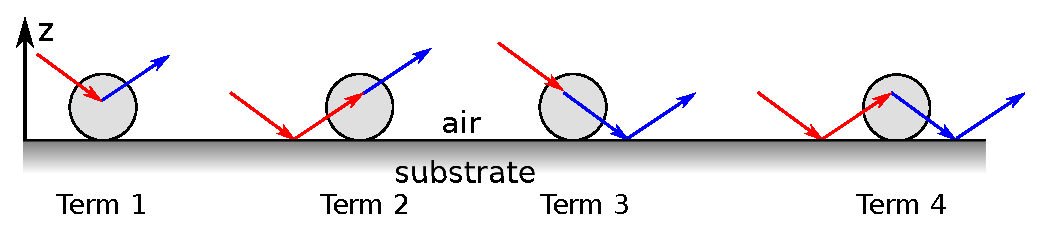
\includegraphics[width=\textwidth]{Figures/drawingDWBA}
\end{center}
\caption{Schematic views of the different terms appearing in the expression of the form factor under DWBA for particles sitting on a substrate layer.}
\label{fig:SchemDWBA}
\end{figure}


Script~\ref{lst:badwba} illustrates the difference between BA and DWBA in \BornAgain\ when generating the sample.  We consider the simple case of:
\begin{itemize}
\item one kind of particles' shape,
\item no interference between the particles,
\item in the DWBA, a sample made of a layer of substrate on which are deposited the particles,
\item in the BA, a sample composed of the particles in air.
\end{itemize} 

Figure~\ref{fig:spheroidbadwba} shows the intensity contourplot generated using this script with truncated spheroids as particles. Note that the full \Python\ script UMFormFactorBA\_DWBA.py is available in /Examples/Python/UserManual/.

\newpage


\begin{lstlisting}[language=python, style=eclipseboxed,numbers=none,nolol,caption={\Code{Python} script to generate a sample using Born or Distorted Wave Born Approximation. The difference between BA and DWBA in this simple case is the absence or presence of a substrate layer in the sample.},label={lst:badwba}]
def get_sample():
    """
    Build and return the sample to calculate form factor of 
    truncated spheroid in Born or Distorted Wave Born Approximation.
    """
    # defining materials
    m_ambience = HomogeneousMaterial("Air", 0.0, 0.0)
    m_substrate = HomogeneousMaterial("Substrate", 6e-6, 2e-8)
    m_particle = HomogeneousMaterial("Particle", 6e-4, 2e-8)

    # collection of particles
    ff= FormFactorTruncatedSpheroid(7.5*nanometer, 9.0*nanometer, 1.2)
    particleshape = Particle(m_particle, ff)
    particle_layout = ParticleLayout()
    particle_layout.addParticle(particleshape, 0.0, 1.0)

    # interferences
    interference = InterferenceFunctionNone()
    particle_layout.addInterferenceFunction(interference)

    # assembling the sample
    air_layer = Layer(m_ambience)
    air_layer.setLayout(particle_layout)
    substrate_layer = Layer(m_substrate, 0)

    multi_layer = MultiLayer()
    multi_layer.addLayer(air_layer)
    # Comment the following line out for Born Approximation
    multi_layer.addLayer(substrate_layer)
    return multi_layer
\end{lstlisting}


\begin{figure}[ht]
\hfill
\subfigure[Born Approximation]{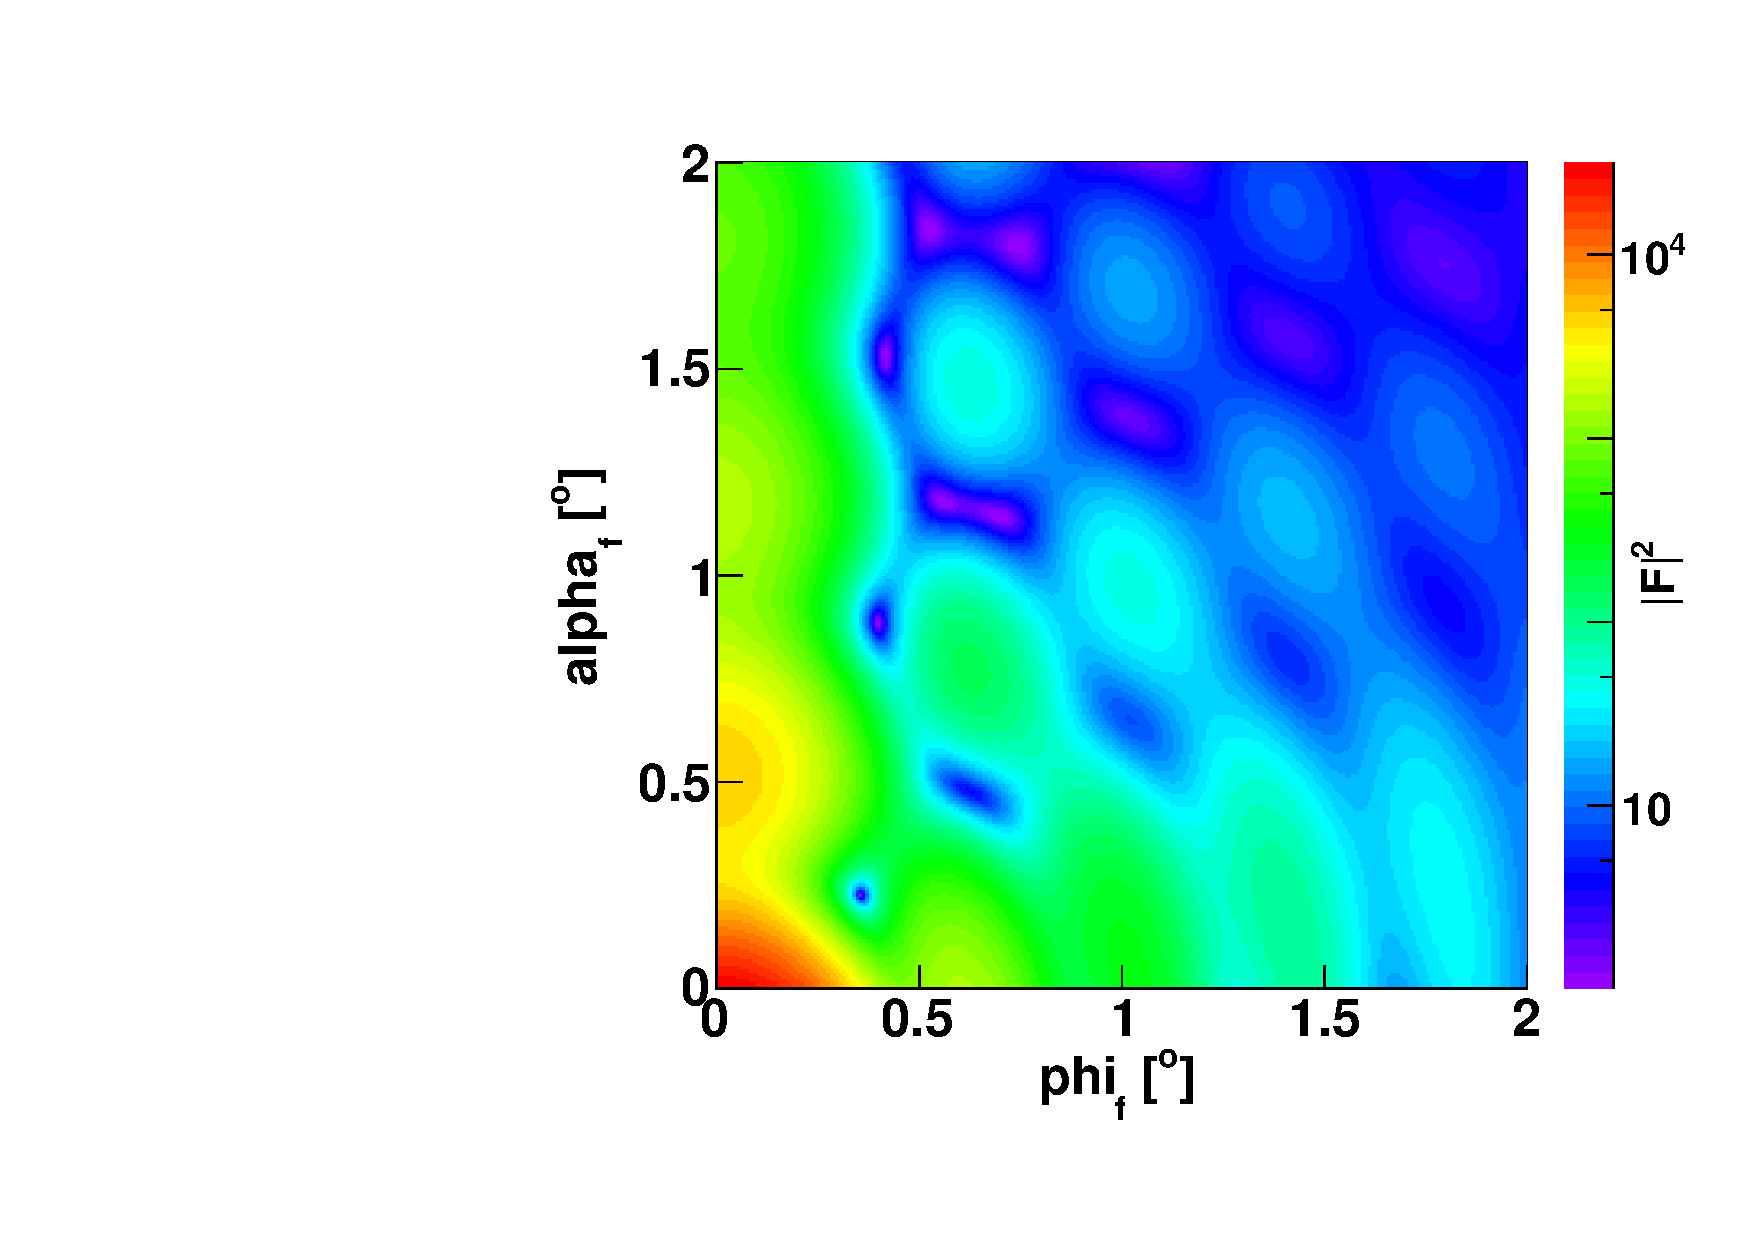
\includegraphics[width=6cm]{Figures/ffspheroidBA}}
\hfill
\subfigure[DWB Approximation]{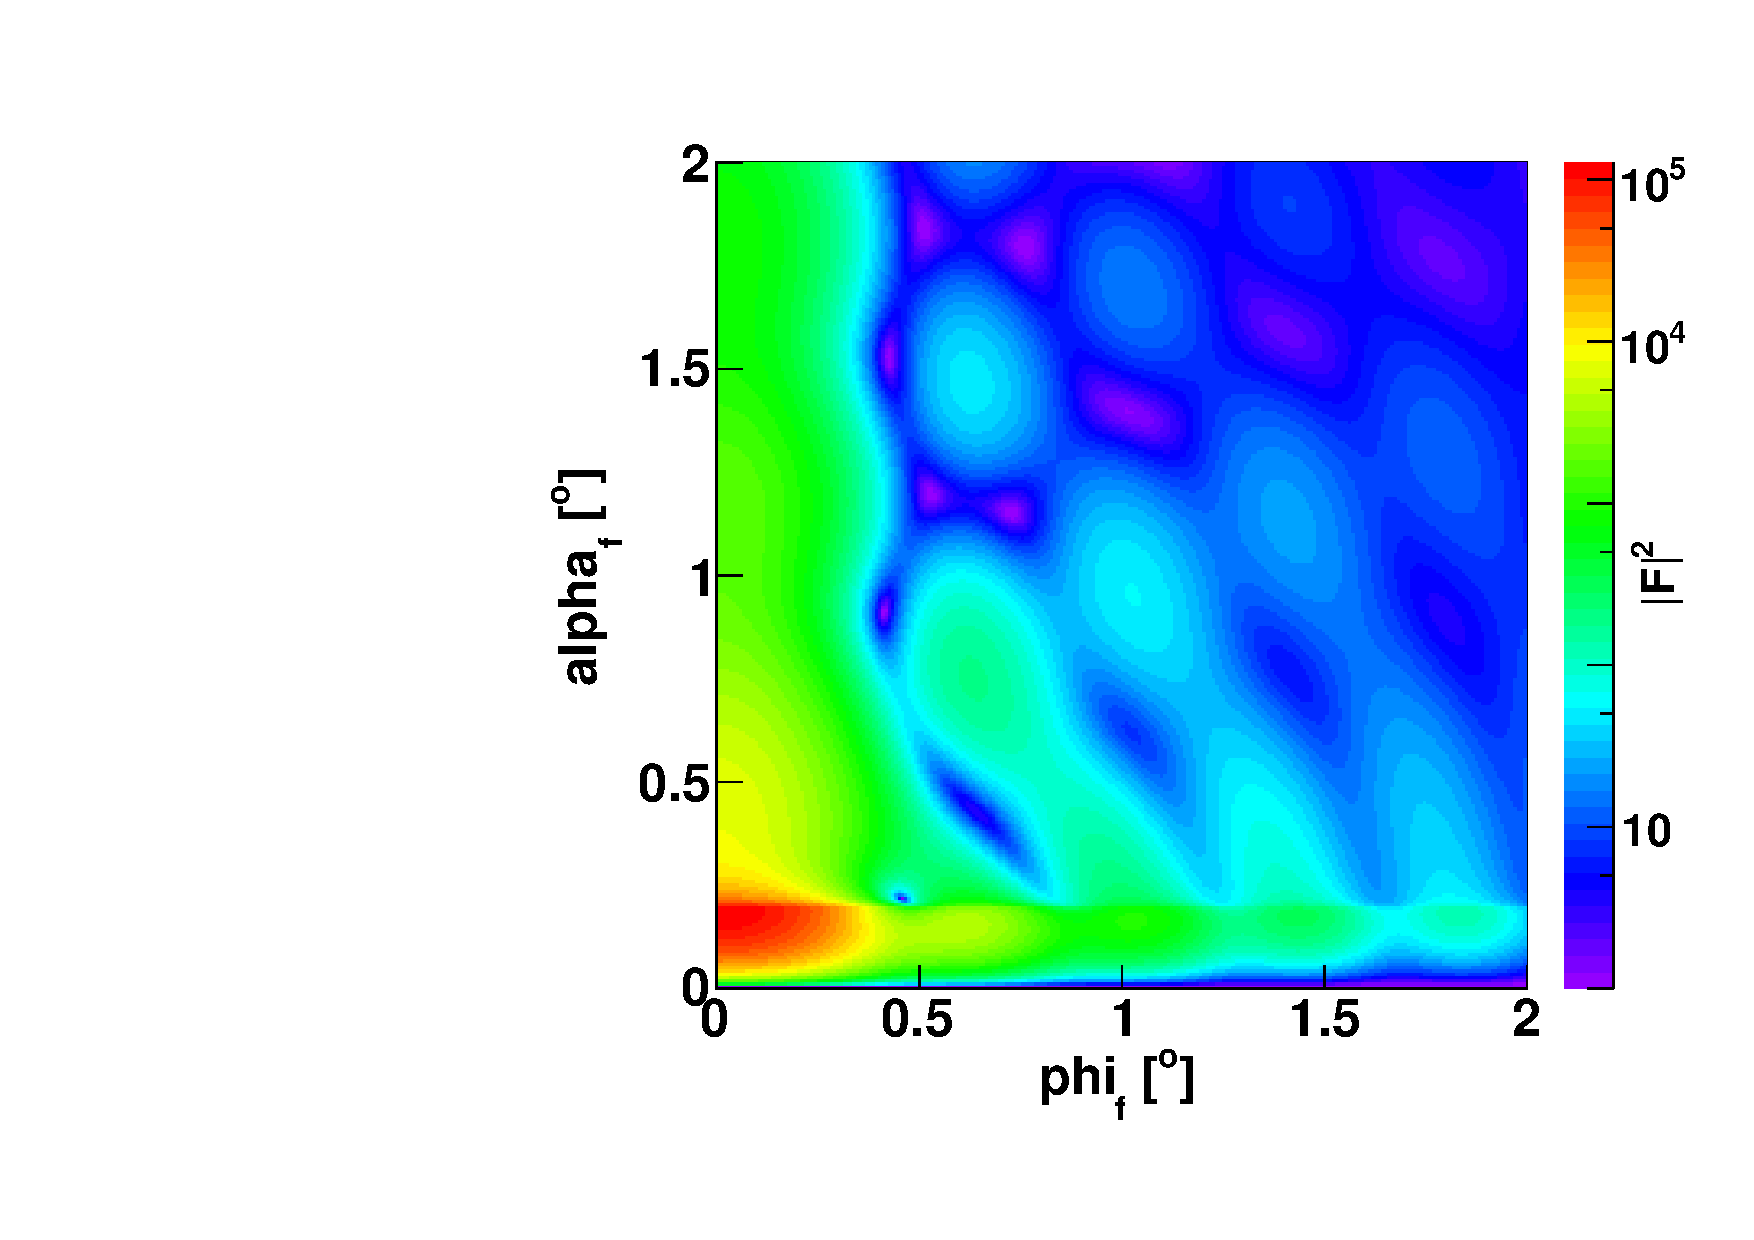
\includegraphics[width=6cm]{Figures/ffspheroidDWBA}}
\hfill
\caption{Intensity map of TruncatedSpheroid form factor in BA and DWBA computing using script~\ref{lst:badwba} for the sample.}
\label{fig:spheroidbadwba}
\end{figure}

\FloatBarrier 

\ImportantPoint{Remark:}{In \BornAgain, the DWBA is implemented automatically when assembling the sample with more than the air layer. The user can nevertheless select between BA or DWBA using \Code{SimulationParameters()} when defining the characteristics of the simulation (it is also the function, with which we can choose between DA, LMA and SSCA).  For example, one could refer to /Examples/Python/UserManual/UM\_FormFactors\_BA\_DWBA\_SimulParam.py for a full implementation:}

\vspace{12pt}

\begin{lstlisting}[language=python, style=eclipseboxed,numbers=none,nolol]
  simulation = Simulation()
  ....
  sim_params = SimulationParameters()
 # choice between BA and DWBA
  sim_params.me_framework = SimulationParameters.DWBA
  ....
  simulation.setSimulationParameters(sim_params)
\end{lstlisting}



\subsubsection{Buried particles} 

The system considered in this section consists of particles encapsulated in a layer, which is sitting on a substrate (see fig.~\ref{fig:SchemDWBAburied}). In this case the form factor in the DWBA is given by

\begin{align}
F_{\rm{DWBA}}(q_{\parallel}, k_{i,z}, k_{f,z}) &= T_i T_f F_{\rm{BA}}(q_{\parallel}, k_{i,z}-k_{f,z})e^{i(k_{i,z}-k_{f,z})d}+ R_i T_f F_{\rm{BA}}(q_{\parallel}, -k_{i,z}-k_{f,z})e^{i(-k_{i,z}-k_{f,z})d} \nonumber \\
&+ R_f T_i F_{\rm{BA}}(q_{\parallel}, k_{i,z}+k_{f,z}) e^{i(k_{i,z}+k_{f,z})d}+ R_f R_iF_{\rm{BA}}(q_{\parallel},-k_{i,z}+k_{f,z})e^{i(-k_{i,z}+k_{f,z})d}, \label{eq:dwbaburied}
\end{align}

\begin{equation*}
R_j =\frac{t^{j}_{0,1}r^{j}_{1,2}\exp(2ik_{j,z}t)}{1+r^{j}_{0,1}r^{j}_{1,2}\exp(2ik_{j,z}t)}, \quad T_j=\frac{t^{j}_{0,1}}{1+r^{j}_{0,1}r^{j}_{1,2}\exp(2ik_{j,z}t)}, j=i,f 
\end{equation*}
where $q_{\parallel}$ is the component of the scattering beam in the plane of the interface, $k_{i,z}$ and $k_{f,z}$ are the z-component of the incident and scattered beams, respectively.  $d$ is the depth at which the particles are sitting in the layer. Note that this value is given relative to the top of this layer and it is not the coordinate in the absolute referential (linked with the full sample) and it is measured up to the bottom of the particle. $t$ is the thickness of the intermediate layer containing the particles. $R_{i,f}$ and $T_{i,f}$  are the reflection  and transmission coefficients in incidence and reflection (they can be calculated using Parratt or matrix formalism). $r^j_{0,1}$, $r^j_{1,2}$ $t^j_{0,1}$ are the reflection and transmission coefficients between layers; the indices are related to different boundaries with 0: air, 1: intermediate layer and 2: substrate layer and the superscript $j$ is associated with the incident or scattered beams:
\begin{equation*}
r^j_{n,n+1}=\frac{k_{j,z,n}-k_{j,z,n+1}}{k_{j,z,n}-k_{j,z,n+1}}, \qquad t^j_{n,n+1}= \frac{2k_{j,z,n}}{k_{j,z,n}-k_{j,z,n+1}}, \quad n=0,1, \quad j=i,f,
\end{equation*}
where index $n$ is related to the layers, $z$ to the vertical component, and $j$ to the beams (incident and outgoing).

\begin{figure}[h]
\begin{center}
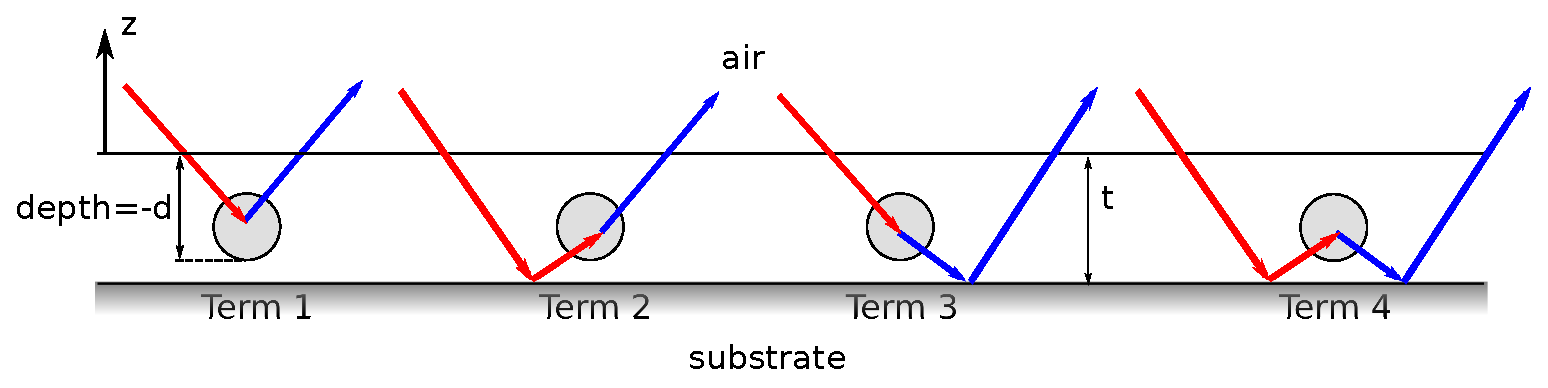
\includegraphics[width=\textwidth]{Figures/drawingDWBAburied}
\end{center}
\caption{Schematic views of the different terms appearing in the expression of the form factor under the DWBA for buried particles.}
\label{fig:SchemDWBAburied}
\end{figure}



Figure~\ref{fig:dwbaburied} shows a typical example of the output intensity scattered from a sample made of 3 layers: air, substrate, and in between, spherical particles embedded in the middle of a 30~nm-thick layer. This figure had been generated using listing~\ref{lst:dwbaburied} (The full script UMFormFactor\_Buried\_DWBA.py can be found in /Examples/Python/UserManual.

\begin{lstlisting}[language=python, style=eclipseboxed,numbers=none,nolol,caption={\Code{Python} script to generate a sample where spherical particles are embedded in the middle of a layer on a substrate.},label={lst:dwbaburied}]
def get_sample():
    """
    Build and return the sample with buried spheres in DWBA.
    """
    # defining materials
    m_ambience = HomogeneousMaterial("Air", 0.0, 0.0)
    m_interm_layer = HomogeneousMaterial("IntermLayer",3.45e-6, 5.24e-9)
    m_substrate = HomogeneousMaterial("Substrate", 7.43e-6, 1.72e-7)
    m_particle = HomogeneousMaterial("Particle", 0.0, 0.0)

    # collection of particles 
    ff = FormFactorFullSphere(10.2*nanometer)
    particleshape = Particle(m_particle, ff)
    particle_layout = ParticleLayout()
    particle_layout.addParticle(particleshape,20.1,1.0)

    # interferences 
    interference = InterferenceFunctionNone()
    particle_layout.addInterferenceFunction(interference)

    # assembling the sample 
    air_layer = Layer(m_ambience)
    intermediate_layer = Layer(m_interm_layer, 30.*nanometer)
    intermediate_layer.setLayout(particle_layout)
    substrate_layer = Layer(m_substrate, 0)
   
    multi_layer = MultiLayer()
    multi_layer.addLayer(air_layer)
    multi_layer.addLayer(intermediate_layer)
    multi_layer.addLayer(substrate_layer)
    return multi_layer
\end{lstlisting}


\begin{figure}[ht]
\centering
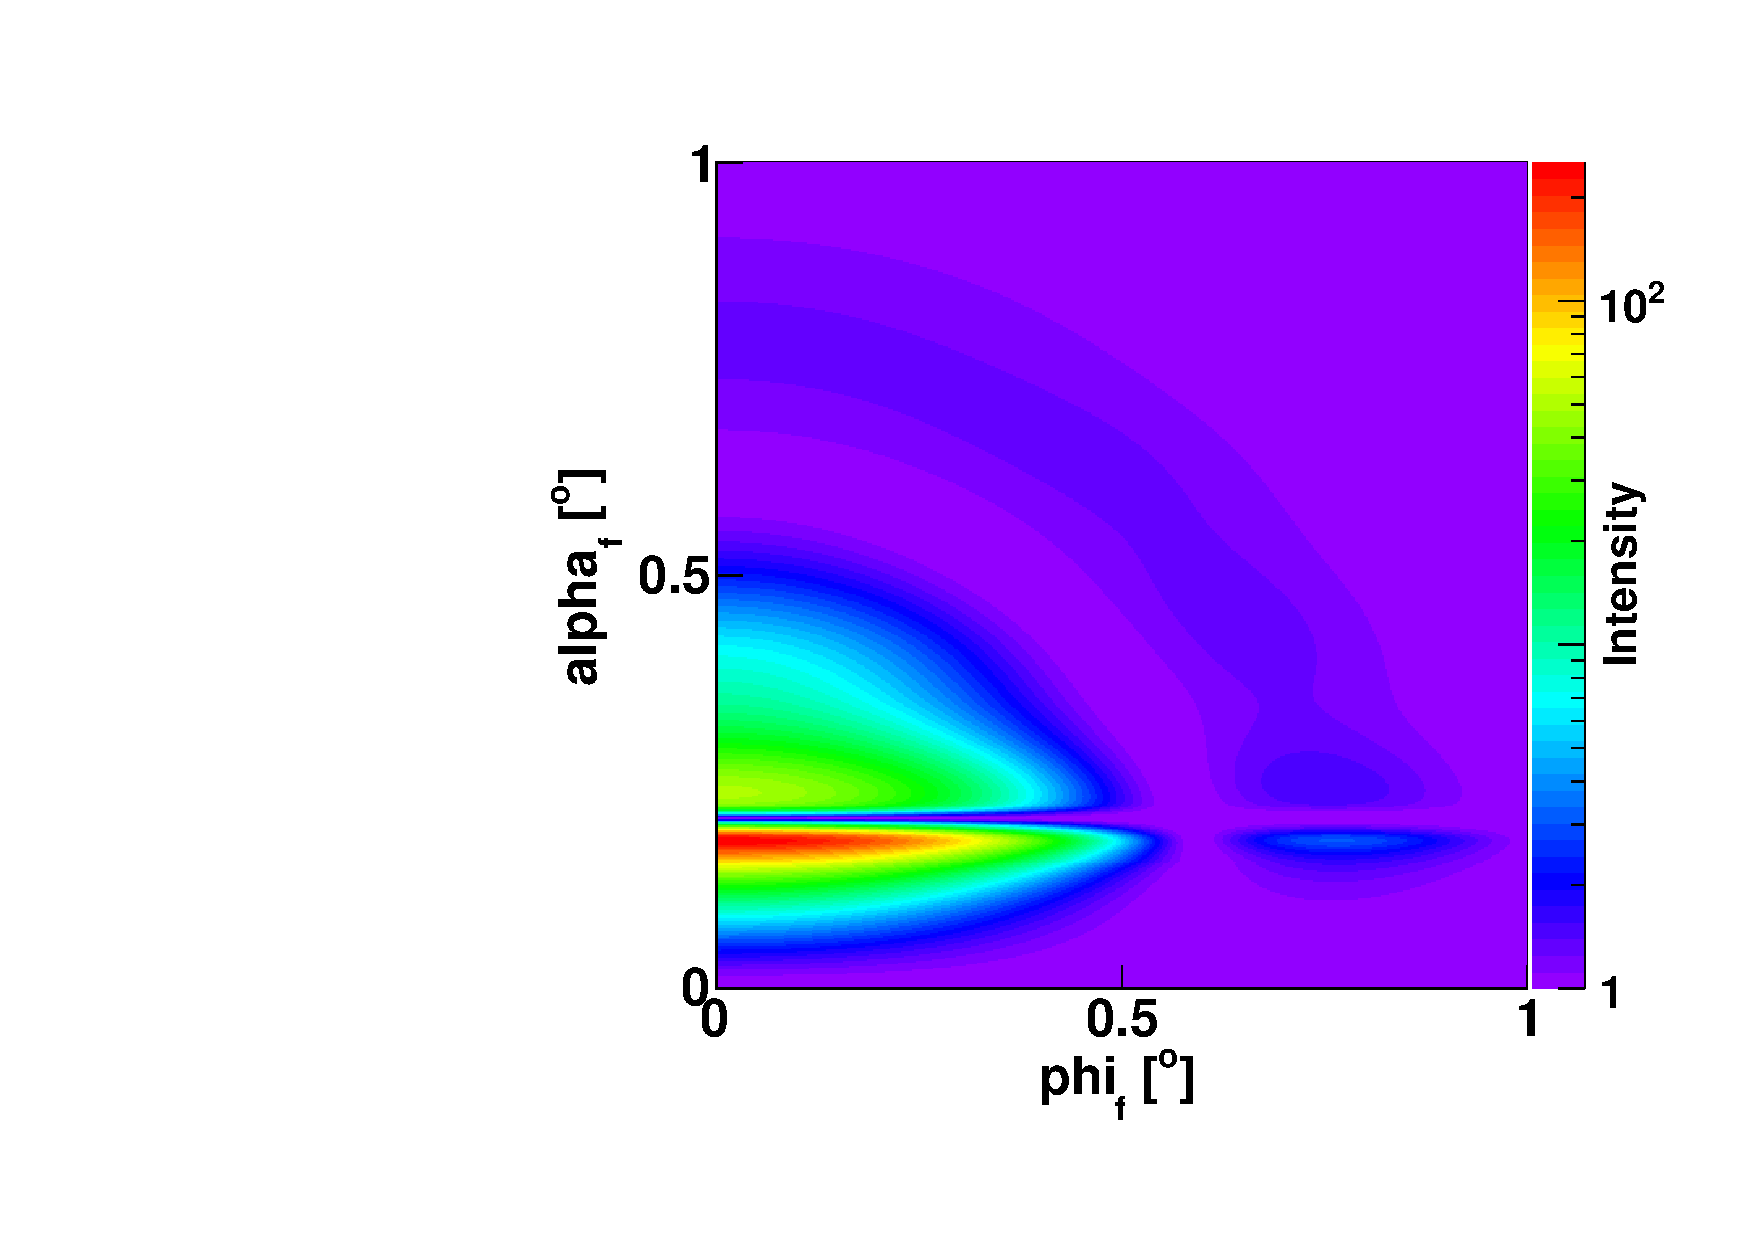
\includegraphics[width=0.6\textwidth]{Figures/figIntBuriedPart}
\caption{Map of intensity scattered from a sample made of spherical particles embedded in the middle of a 30~nm-thick layer on a substrate (see Script~\ref{lst:dwbaburied} for details about the sample).}
\label{fig:dwbaburied}
\end{figure}

\newpage

\ImportantPoint{Remark:}{For layers different from the air layer, the top interface is considered as the reference level to position the encapsulated particles. For example, spheres positioned at depth $d$ (positive) are located at a distance $d$ from the top of the layer up to the bottom of these particles. This convention is different for the top air layer, where particles sitting at the interface with an underlying layer (\textit{i.e.} the bottom of the air layer) are located at depth 0 (see fig.~\ref{fig:depthpartBA}).}


\begin{figure}[ht]
\centering
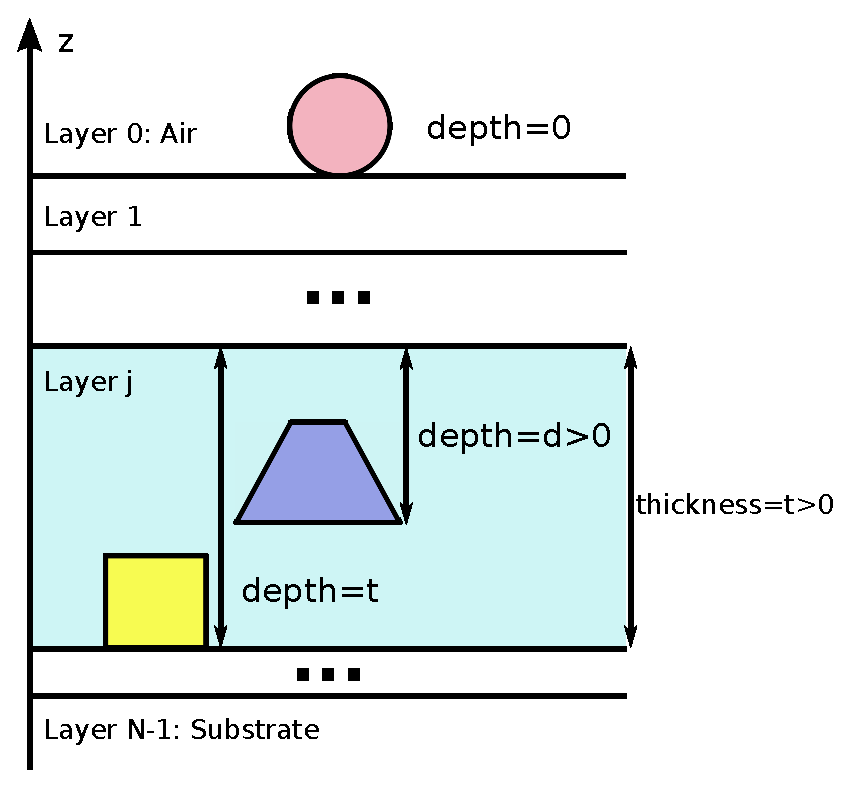
\includegraphics[width=0.5\textwidth]{Figures/drawingDepthParticle}
\caption{Illustration of the convention about \Code{depth} used in \BornAgain\ to encapsulate particles in layers.}
\label{fig:depthpartBA}
\end{figure}


\newpage
%%%%%%%%%%%%%%%%%%%%%%%%%%%%%%%%%%%%%%%%%
\section{More complicated particles' shapes} 
\BornAgain\ also offers the possibility to simulate more complicated shapes of particles by combining those listed in Table~\ref{tab:formfactors}. 

\subsection{Core-shell particles}
 To generate a core-shell particle, the combination is performed using the following command:\\
\Code{ParticleCoreShell(shell\_particle, core\_particle, relative\_core\_position)},\\
where \Code{shell\_particle} and \Code{core\_particle} are the outer and inner parts of the core-shell particle, respectively. They refer to one of the form factors defined previously and to an associated material. For example, for the outer part,\\ \Code{shell\_particle=Particle(material\_shell, outer\_form\_factor)},\\ where \Code{material\_shell} is the material of the shell and \Code{outer\_form\_factor} is the shape of the outer part (cf. listing~\ref{lst:cshellsample}). \\ \Code{relative\_core\_position} defines the position of the centre of gravity of the inner shape with respect to the outer one. An example in fig.~\ref{fig:coreshell} shows a core shell particle made of a box for the outer part and of a shifted pyramidal shape for the inner one.\\

Figure~\ref{fig:FFCoreShellBA} displays the output intensity scattered in the Born Approximation using the code listed in~\ref{lst:cshellsample} to generate the core-shell particle. The full script can be found at /Examples/python/UserManual/UMFormFactor\_CoreShell.py. 

\begin{figure}[ht]
\hfill
\subfigure[Side view]{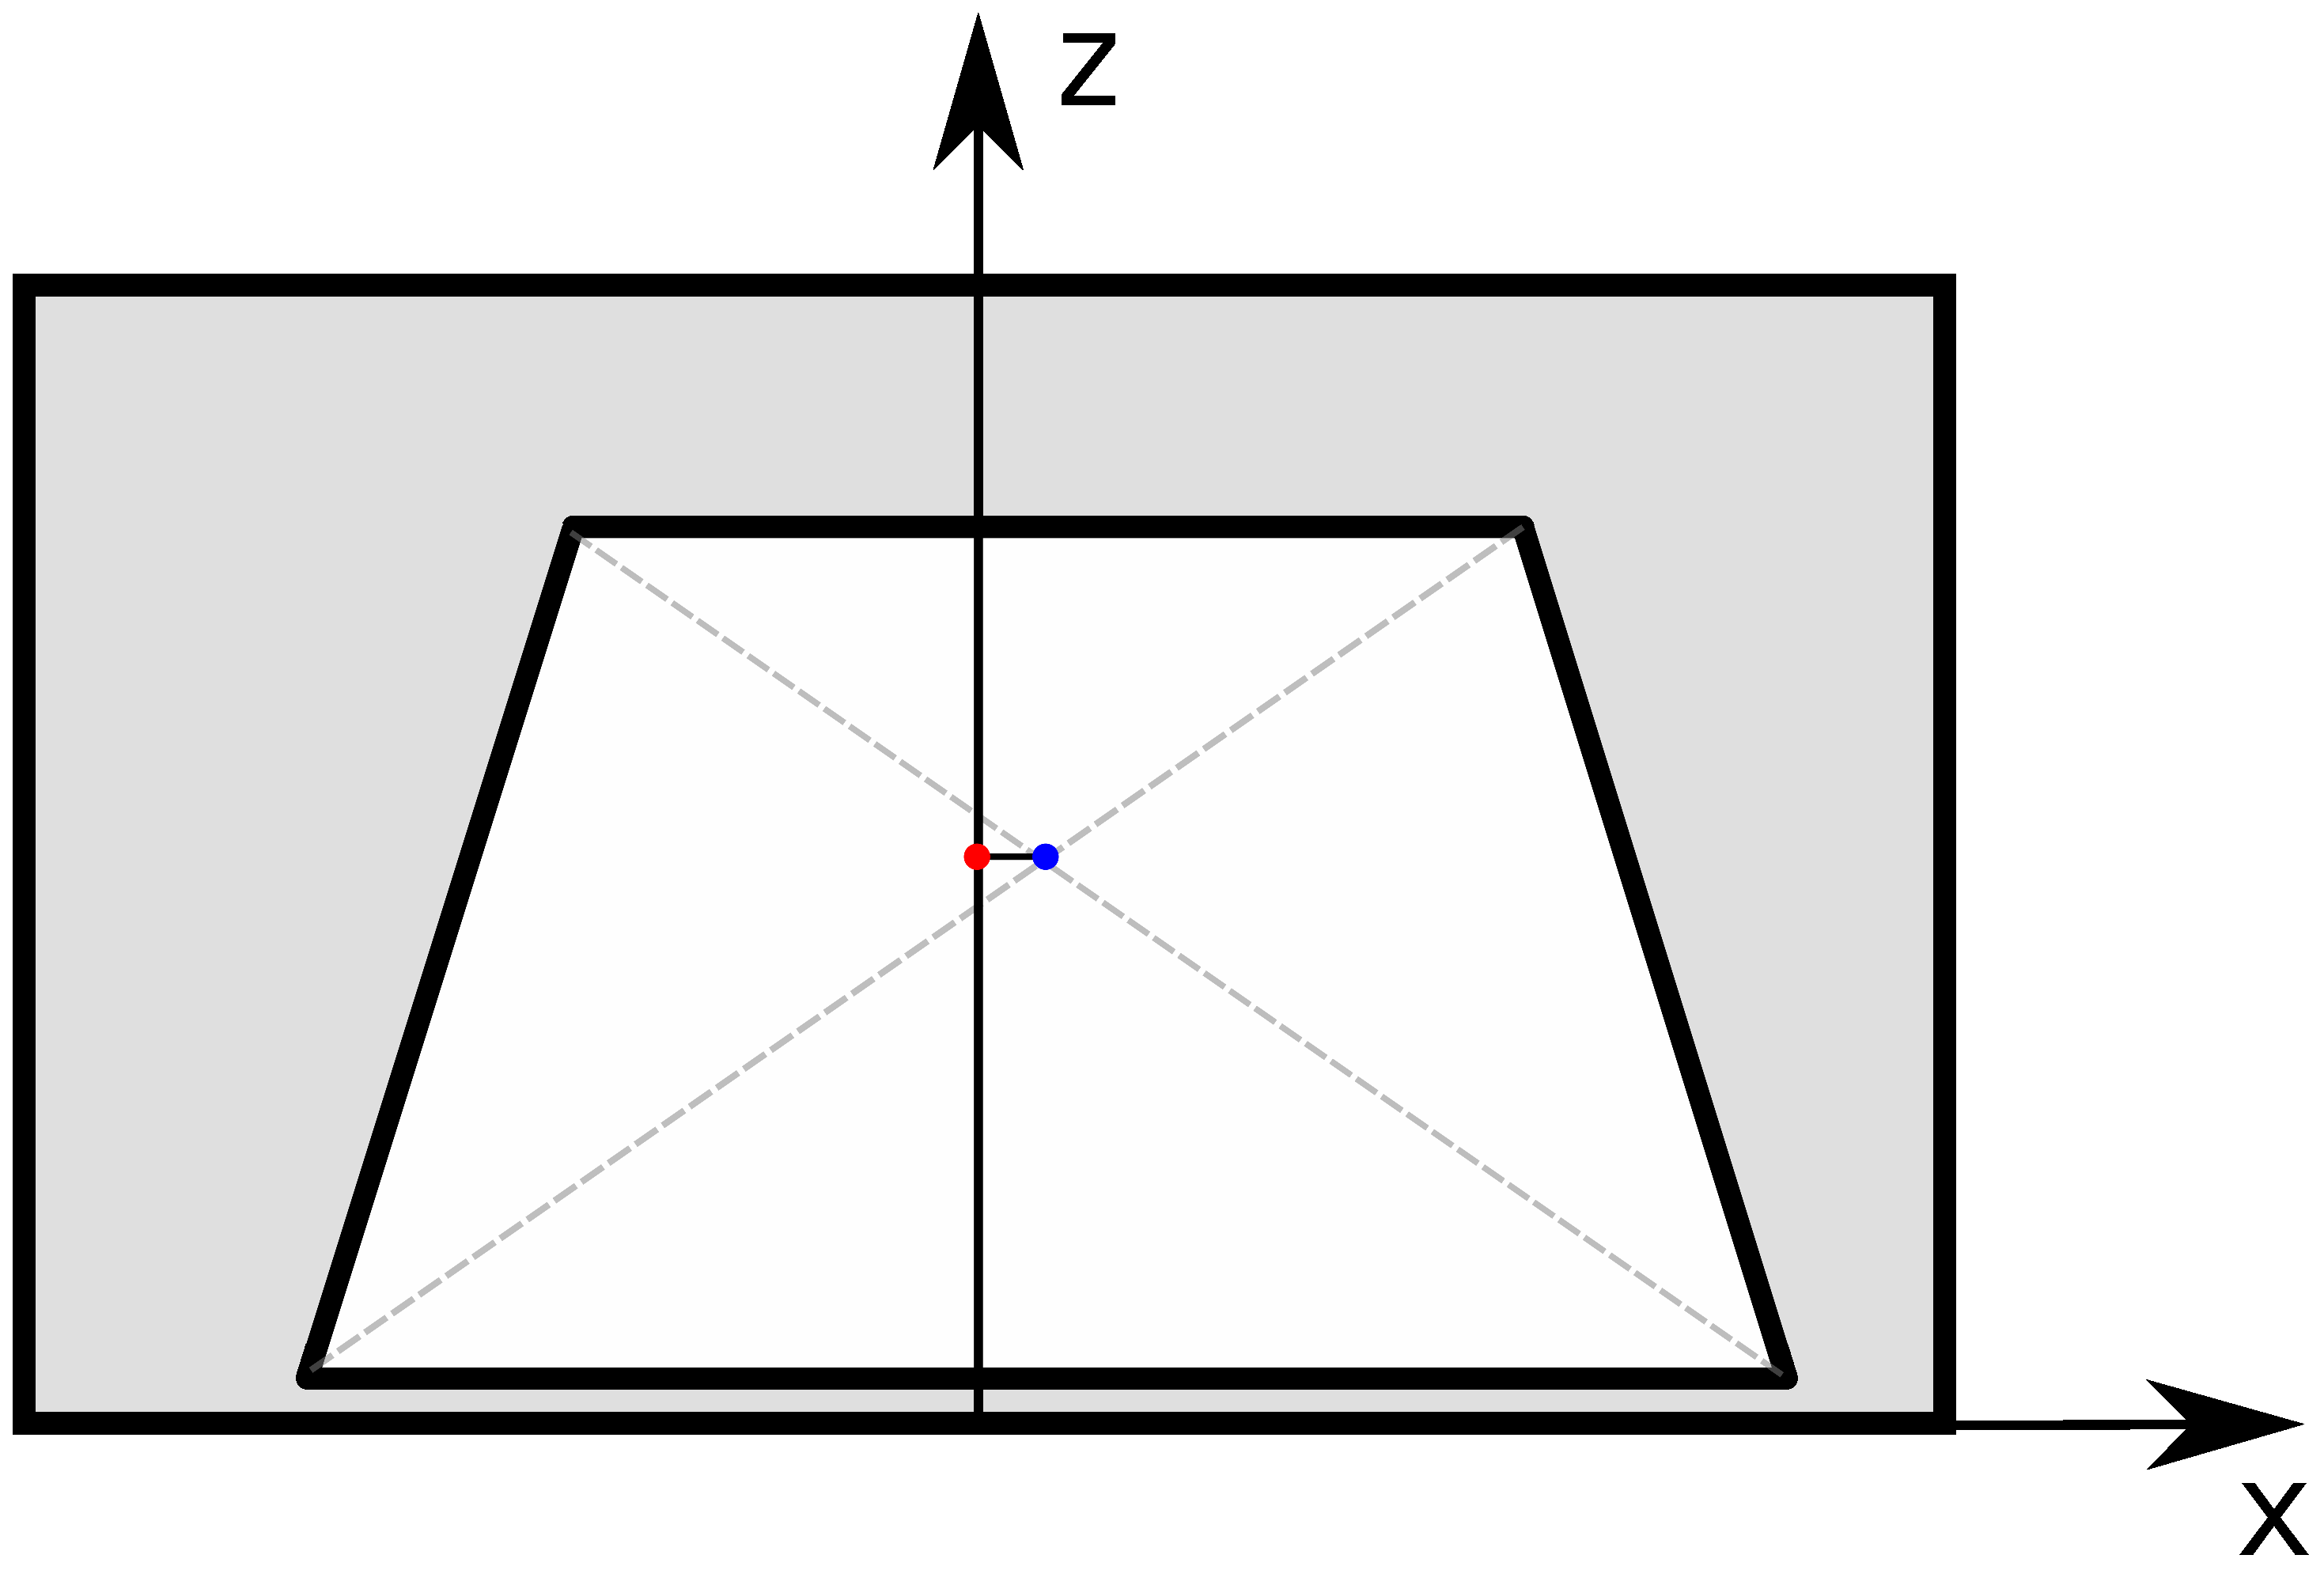
\includegraphics[width=5cm]{Figures/CoreShellParallPyrxz}}
\hfill
\subfigure[Top view]{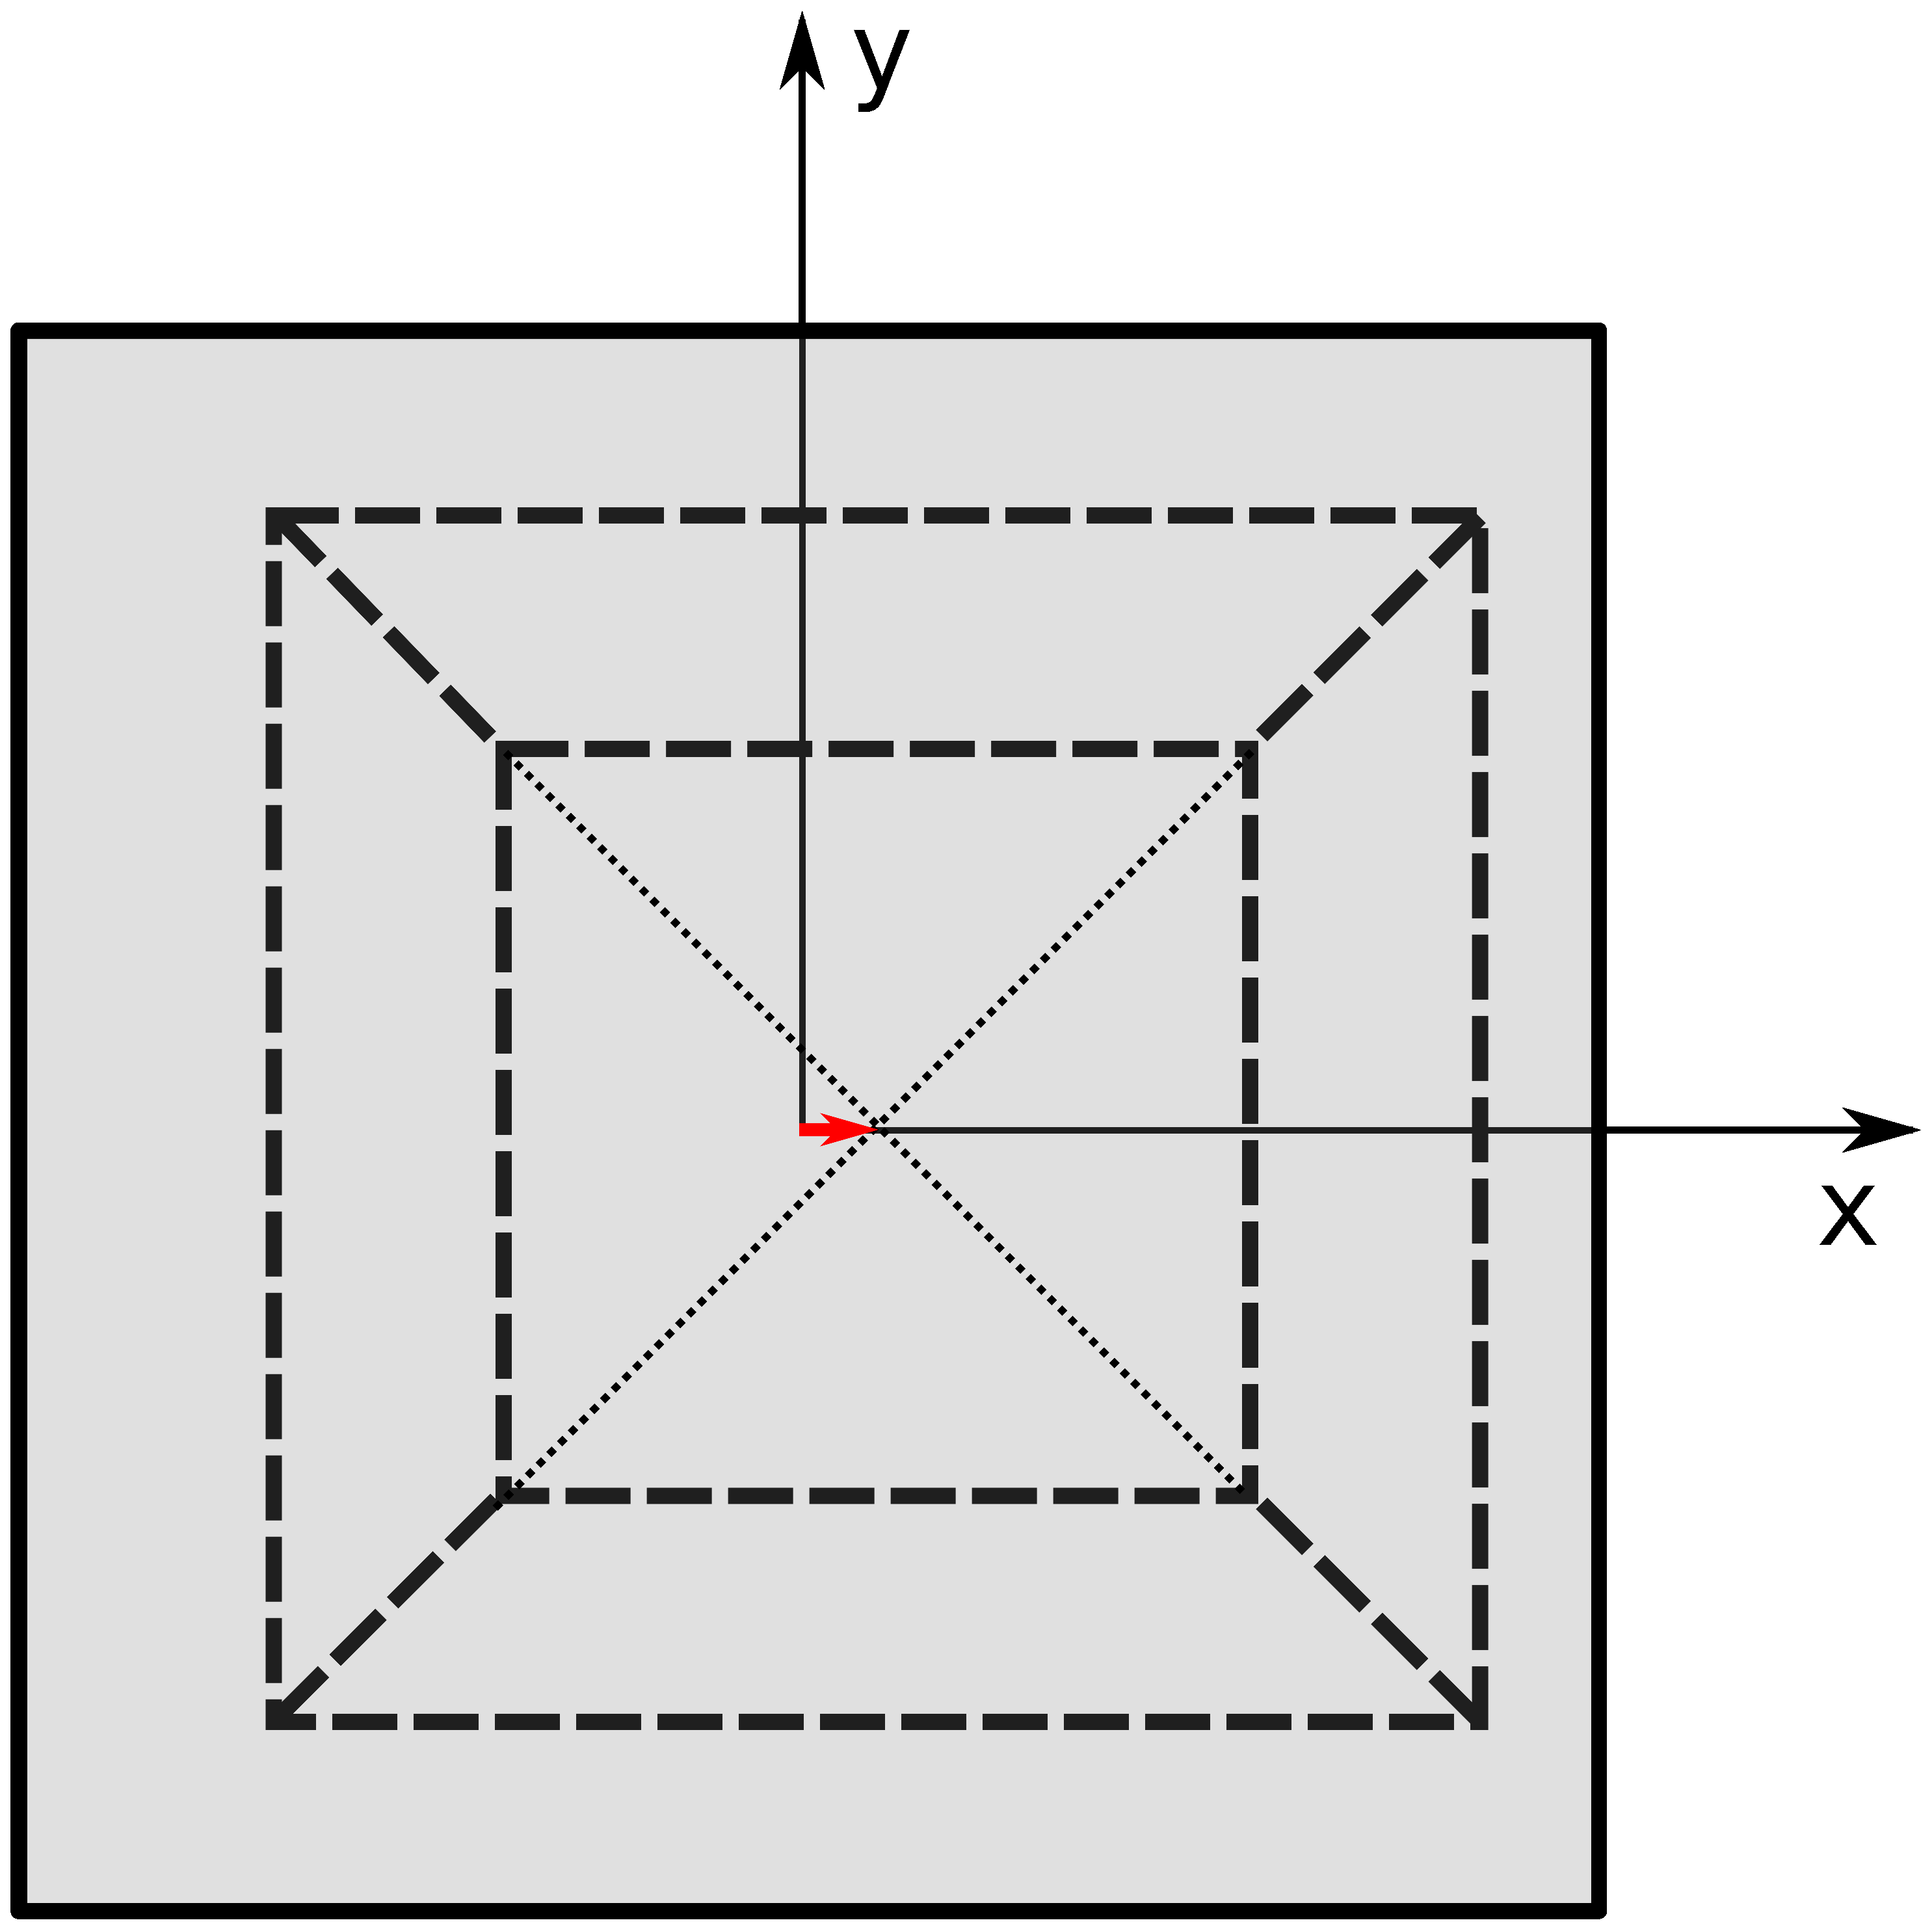
\includegraphics[width=5cm]{Figures/CoreShellParallPyrxy}}
\hfill
\caption{Example of a core-shell particle composed of a box with a pyramidal  inset. The relative core shell position is marked by the position of its center of gravity (blue point $\color{blue}\bullet$) with respect to the center of gravity of the box (red point $\color{red}\bullet$). }
\label{fig:coreshell}
\end{figure}

\newpage


\begin{lstlisting}[language=python,
  style=eclipseboxed,numbers=none,nolol,caption={\Code{Python} script
    to create a core-shell particle made of a box with a pyramidal shifted inset.},label={lst:cshellsample}]
    outer_ff = FormFactorBox(16.0*nanometer, 16.0*nanometer, 8.0*nanometer) 
    inner_ff = FormFactorPyramid(12.0*nanometer, 7.0*nanometer, 60.0*degree)
    shell_particle = Particle(m_shell, outer_ff)
    core_particle = Particle(m_core, inner_ff)
    core_position = kvector_t(1.5, 0.0, 0.0)

    particle = ParticleCoreShell(shell_particle, core_particle, core_position)
\end{lstlisting}

\begin{figure}[h]
\begin{center}
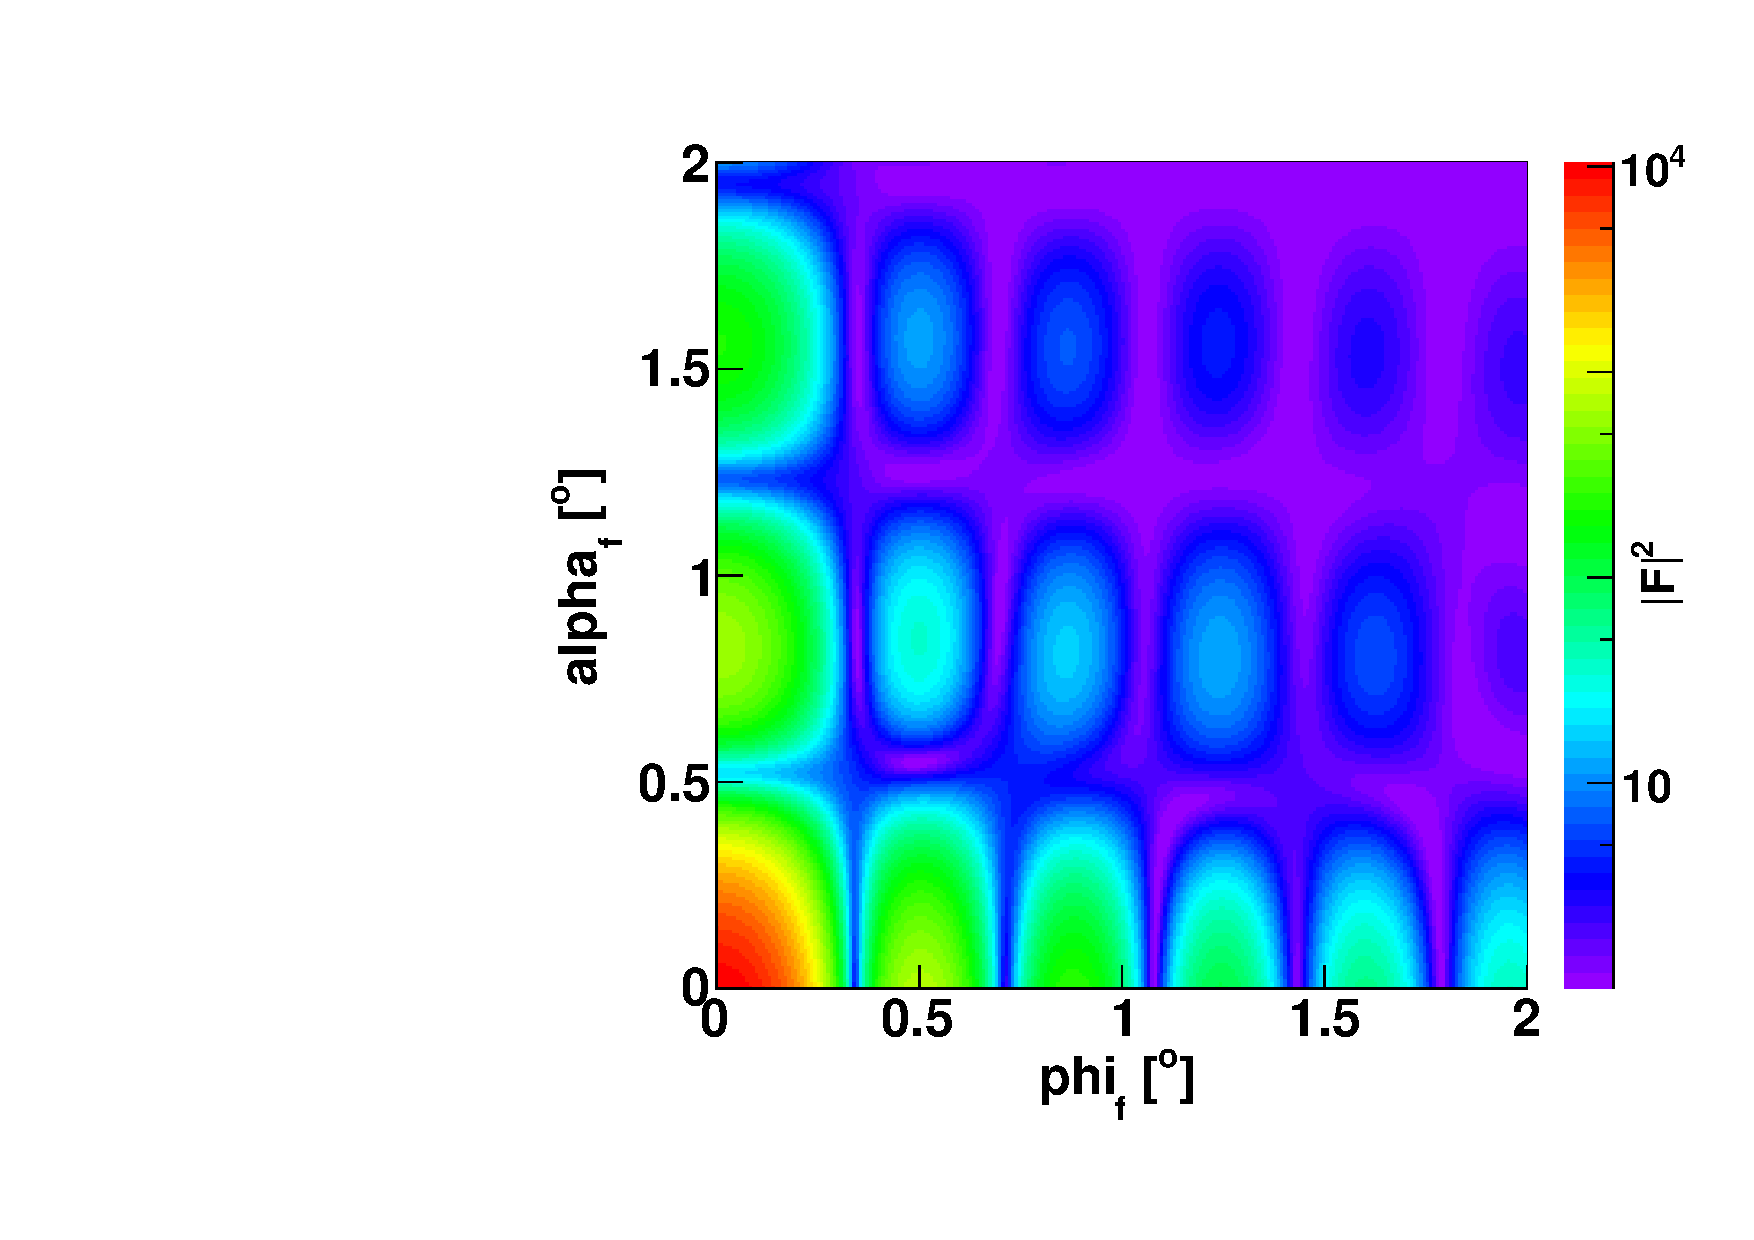
\includegraphics[width=0.6\textwidth]{Figures/CoreShellParallPyr}
\end{center}
\caption{Intensity map of a core-shell form factor in Born Approximation using  \Code{FormFactorBox(16*nanometer, 16*nanometer, 8*nanometer)} and \Code{FormFactorPyramid(12*nanometer, 7*nanometer, 60*degree)} for the outer and inner shells, respectively. The core particle is shifted by 1.5~nm in the $x$-direction with respect to the centre of the outer shell. The sample used to generate the particle is listed in~\ref{lst:cshellsample}.  There is no substrate and no interference between the particles.}
\label{fig:FFCoreShellBA}
\end{figure}

%%%%%%%%%%%%%%%%%%%%%%%%%%%%%%%%%%%%%%%%%
\subsection{Rotation of particles}

The particles can be rotated in a different direction by using one of
the following transformations: \Code{CreateRotateX($\theta$),
  CreateRotateY($\theta$), CreateRotateZ($\theta$)}, where capital X, Y, Z mark rotations
around the associated axis and $\theta$ is the
angle of rotation from this axis. For example, the following \Code{Python}\ script shows how to rotate a pyramid by $45^{\circ}$ around
the $z$-axis:\\

\begin{lstlisting}[language=python, style=eclipseboxed,numbers=none,nolol]
    pyramid_ff = FormFactorPyramid(10*nanometer, 5*nanometer, deg2rad(54.73 ) )
    pyramid = Particle(m_particle, pyramid_ff)
    angle_around_z = 45.*degree
    transform = Transform3D.createRotateZ(angle_around_z)
    particle_layout = ParticleLayout()
    particle_layout.addParticle(pyramid, transform) 
\end{lstlisting}

\subsection{Polydispersity}

%%%%%%%%%%%%%%%%%%%%%%%%%%%%%%%%%%%%%%%%%
\section{Material layers}
\subsection{Roughness}
\section{Polarisation}
To be completed 
